\documentclass{ieeeojies}
\usepackage{cite}
\usepackage{amsmath,amssymb,amsfonts}
\usepackage{algorithmic}
\usepackage{graphicx}
\usepackage{textcomp}
\usepackage{array}
\usepackage[table]{xcolor}
\usepackage{multirow}
\usepackage{multicol}
\usepackage{float}

\def\BibTeX{{\rm B\kern-.05em{\sc i\kern-.025em b}\kern-.08em
    T\kern-.1667em\lower.7ex\hbox{E}\kern-.125emX}}

\begin{document}
\title{\centering\LARGE\MakeUppercase{Forecasting of bank's stock price using using statistic model, machine learning and deep learning}}

\author{\uppercase{Dang Quang Nhat}\authorrefmark{1},
\uppercase{Tran Phuc Thinh\authorrefmark{2}, and Nguyen Dai Duong}\authorrefmark{3}}

\address[1]{21522413, Faculty of Information Systems, University of Information Technology, (e-mail: 21522413@gm.uit.edu.vn)}
\address[2]{21521475, Faculty of Information Systems, University of Information Technology, (e-mail: 21521475@gm.uit.edu.vn)}
\address[3]{21520756, Faculty of Information Systems, University of Information Technology, (e-mail: 21520756@gm.uit.edu.vn)}

\markboth
{Author \headeretal: Dang Quang Nhat, Tran Phuc Thinh, Nguyen Dai Duong}
{Author \headeretal: Dang Quang Nhat, Tran Phuc Thinh, Nguyen Dai Duong}

\begin{abstract} \par
 \textbf{Forecasting stock market trends is crucial for investment decision-making, especially in the Vietnamese banking sector. This scientific report examines the application of statistical models and machine learning techniques to predict the future movements of three major Vietnamese bank stocks.Eight forecasting models, including ARIMA, GRU, linear regression, GARCH, MICN, RNN, LSTM, and GradientBoosting, provide valuable insights into the dynamics and trends within this crucial sector of the Vietnamese economy. The findings are expected to contribute to the existing knowledge on stock market forecasting and inform the development of investment strategies and risk management practices in the Vietnamese banking stock market.}\\

\textit{\textbf{INDEX TERMS:}bank stocks in Vietnam, stock market forecasting, statistical models, machine learning, neural network, ARIMA, GRU, Linear Regression, GARCH, RNN, MICN, GradientBoosting, LSTM.}
\end{abstract}
\titlepgskip=-15pt
\maketitle

\section{Introduction}
The stock market is characterized as dynamic, unpredictable, and non-linear in nature. Predicting stock prices is a challenging task as it depends on various factors including, but not limited to, political conditions, the global economy, and company financial reports and performance. Thus, to maximize profit and minimize losses, techniques to predict stock values in advance by analyzing trends over the last few years could prove to be highly useful for making stock market movements. \cite{b1} \cite{b2}

\noindent The Vietnamese stock market has witnessed significant growth in recent years. However, accurately forecasting stock prices remains a difficult task due to the inherent complexities of financial markets. This study addresses this challenge by using machine learning and deep learning algorithms to forecast the stock prices of three major Vietnamese banks: Vietcombank, ACB, and VietinBank. This research contributes to the growing body of knowledge concerning financial forecasting in emerging markets by employing advanced computational techniques to analyze and predict stock prices within the dynamic Vietnamese context.

\noindent This research explores how various machine and deep learning algorithms can predict stock prices in Vietnam. The study will test popular algorithms, including Long Short-Term Memory (LSTM) networks, Gated Recurrent Units (GRUs), Recurrent Neural Networks (RNNs), Linear Regression, and Autoregressive Integrated Moving Average (ARIMA) models, to determine their effectiveness in capturing stock price trends. Each algorithm's unique strengths in modeling stock prices will be evaluated using performance metrics such as Mean Absolute Percentage Error (MAPE) and Root Mean Square Error (RMSE).

\noindent To further improve accuracy the study will experiment with advanced techniques such as MICN (Multi-scale Isometric Convolution Network), Gradient Boosting Regressors, and Generalized Autoregressive Conditional Heteroskedasticity (GARCH) models.

\noindent Overall, this research aims to improve the accuracy of stock price predictions in Vietnam's stock market using machine and deep learning models. By making these predictions more reliable, investors and other stakeholders can make smarter investment decisions.

\label{sec:introduction}
 

\section{Related Works}
The application of machine learning and deep learning algorithms to stock price prediction has garnered significant attention in recent years. Various studies have explored different models and techniques to enhance prediction accuracy and reliability.
Most previous work in this area utilizes classical algorithms like linear regression \cite{b3} and linear models such as Autoregressive Integrated Moving Average (ARIMA) \cite{b4} for predicting stock prices.
Some techniques based on neural networks, such as Convolutional Neural Networks (CNN), Recurrent Neural Networks (RNN), and deep neural networks like Long Short-Term Memory (LSTM), have also shown promising results \cite{b5}\cite{b6}.
Recent advancements in stock forecasting have seen a rise in the use of Gated Recurrent Units (GRUs). Studies have compared GRU models to other methods like Support Vector Machines (SVM) for predicting trading signals based on stock indicators \cite{b7}
Recurrent Neural Networks (RNNs), particularly Long Short-Term Memory (LSTM) networks, have proven effective in time series forecasting. LSTMs excel at capturing long-term dependencies within data, making them suitable for analyzing historical trends alongside current data for stock price prediction \cite{b8}\cite{b9}. In recent years, researchers have applied LSTMs to various stock markets globally. For example, Chen et al. \cite{b10} utilized LSTMs to forecast China's Shanghai and Shenzhen stock markets.
In addition to traditional neural networks, advanced techniques like Gradient Boosting Regressors and Generalized Autoregressive Conditional Heteroskedasticity (GARCH) models have been explored. Gradient Boosting is an ensemble technique that builds multiple weak learners, usually decision trees, to improve predictive accuracy. GARCH models are used to predict volatility in financial markets and have been integrated with other predictive models to enhance performance. Kim, Jong-Min  et al \cite{b11}. Comparing the Performances of GARCH-type Models in Capturing the Stock Market Volatility in Malaysia 
Gradient Boosting has been extensively applied in financial time-series modeling due to its ability to handle complex, non-linear relationships within data. Regularised Gradient Boosting, in particular, has shown promise in improving predictive accuracy and robustness. Agapitos, Brabazon, and O’Neill (2017) \cite{b12} explored the application of Regularised Gradient Boosting for financial time-series modeling. Their study highlighted the advantages of using gradient boosting algorithms in capturing the intricate patterns present in financial data
The Multi-scale Isometric Convolution Network (MICN) model by Wang et al. (2022) \cite{b13} represents a significant advancement in long-term series forecasting. MICN integrates multi-scale local and global context modeling to effectively capture complex patterns and dependencies within time-series data.

Prior to MICN, Convolutional neural networks (CNN) are widely used in computer vision, natural language processing and speech recognition. Meanwhile, Transformer architectures (Vaswani et al., 2017) \cite{b14} introduced attention mechanisms for learning intricate temporal relationships across different scales.

MICN distinguishes itself by leveraging multi-scale isometric convolutions, which enhance its ability to handle both short-term fluctuations and long-term trends in time-series forecasting. This approach improves prediction accuracy and interpretability, making MICN suitable for applications in finance, climate science, and healthcare.

\section{Materials}
\subsection{Dataset}
Datasest 
We will be analyzing historical stock data for Joint Stock Commercial Bank For Foreign Trade Of Vietnam (VCB), Asia Commercial Joint Stock Bank (ACB), and Vietnam Joint Stock Commercial Bank for Industry and Trade (CTG), covering the period from March 1st, 2019 to June 10th, 2024. The dataset includes columns such as Date, Open, High, Low, Close, Adj Close, and Volume. Our focus will be on processing the "Close" price for forecasting purposes.

\subsection{Descriptive Statistics}
\begin{table}[H]
  \centering
  \caption{VCB, ACB, CTG’s Descriptive Statistics}
\begin{tabular}{|>{\columncolor{red!20}}c|c|c|c|}
    \hline
     \rowcolor{red!20} & VCB & ACB & CTG \\ \hline
     Count & 1311 & 1313 & 1317 \\ \hline
     Mean & 66758.246 & 15745.649& 23713.87\\ \hline
     Std & 13660.147 & 5246.805 & 6526.769\\ \hline
     Min & 37957.312 & 6626.145 & 11925.876\\ \hline
     25\% & 56604.175 & 9157.481 & 16710.095\\ \hline
     50\% & 65198.984 & 18071.833 & 25192.072\\ \hline
     75\% & 75867.910 & 19608.695 & 28635.972\\ \hline
     Max & 97400 & 25782.609 & 37719.05\\ \hline
\end{tabular}
\end{table}

\begin{figure}[H]
    \centering
    \begin{minipage}{0.23\textwidth}
    \centering
    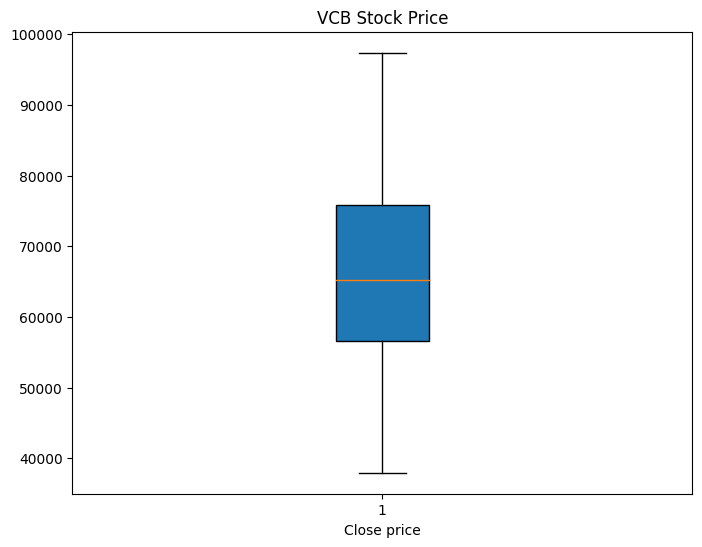
\includegraphics[width=1\textwidth]{bibliography/boxplot_vcb.png}
    \caption{VCB stock price's boxplot}
    \label{fig:1}
    \end{minipage}
    \hfill
    \begin{minipage}{0.23\textwidth}
    \centering
    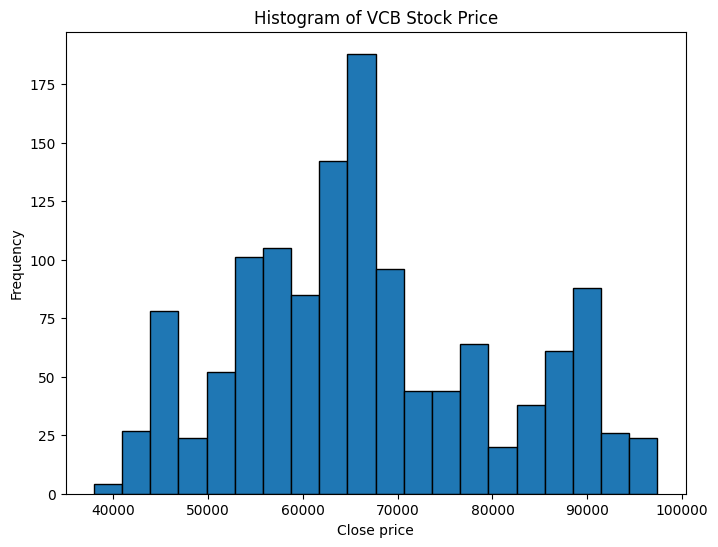
\includegraphics[width=1\textwidth]{bibliography/histogram_vcb.png}
    \caption{VCB stock price's histogram}
    \label{fig:2}
    \end{minipage}
\end{figure}

\begin{figure}[H]
    \centering
    \begin{minipage}{0.23\textwidth}
    \centering
    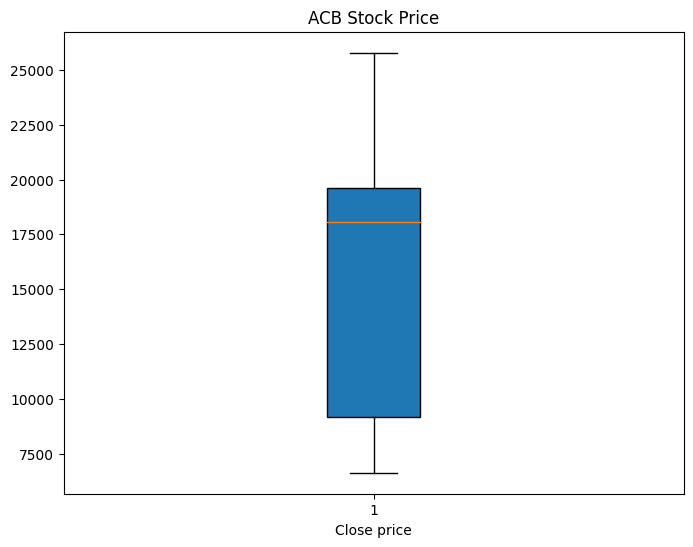
\includegraphics[width=1\textwidth]{bibliography/boxplot_acb.png}
    \caption{ACB stock price's boxplot}
    \label{fig:1}
    \end{minipage}
    \hfill
    \begin{minipage}{0.23\textwidth}
    \centering
    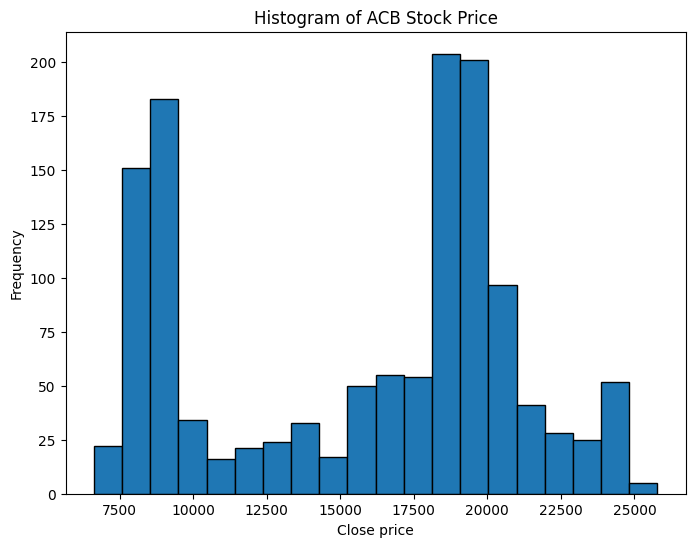
\includegraphics[width=1\textwidth]{bibliography/histogram_acb.png}
    \caption{ACB stock price's histogram}
    \label{fig:2}
    \end{minipage}
\end{figure}

\begin{figure}[H]
    \centering
    \begin{minipage}{0.23\textwidth}
    \centering
    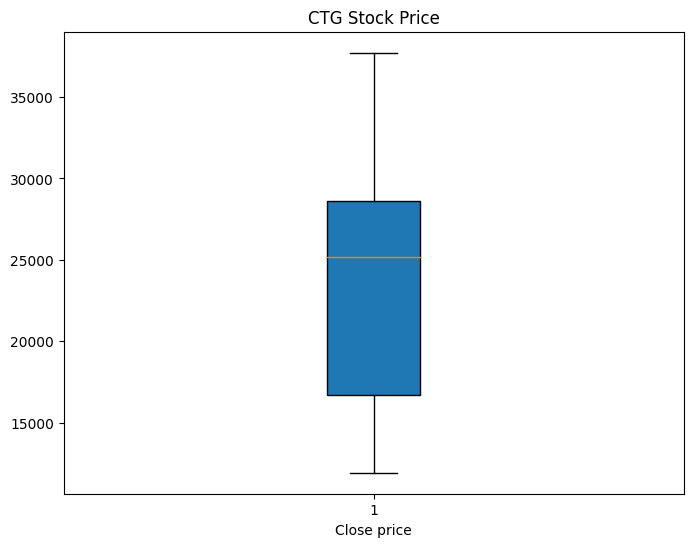
\includegraphics[width=1\textwidth]{bibliography/boxplot_ctg.png}
    \caption{CTG stock price's boxplot}
    \label{fig:1}
    \end{minipage}
    \hfill
    \begin{minipage}{0.23\textwidth}
    \centering
    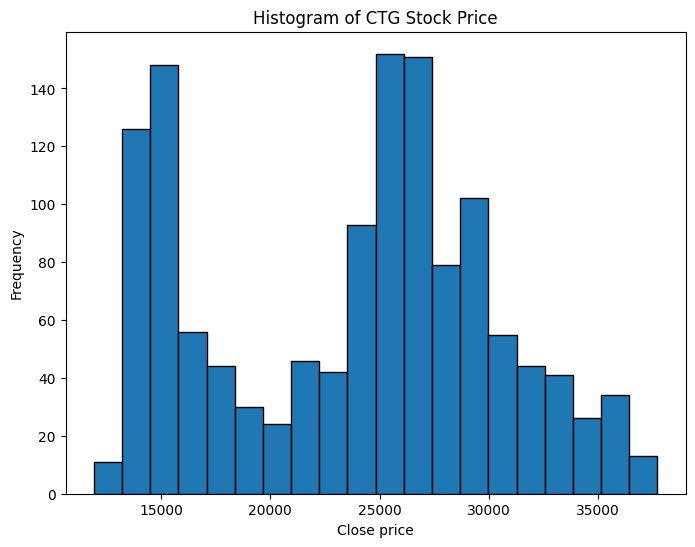
\includegraphics[width=1\textwidth]{bibliography/histogram_ctg.png}
    \caption{CTG stock price's histogram}
    \label{fig:2}
    \end{minipage}
\end{figure}

\section{Methodology}
\subsection{Linear Regression}
Linear regression is a statistical procedure for calculating the value of a dependent variable from an independent variable. Linear regression measures the association between two variables. It is a modeling technique where a dependent variable is predicted based on one or more independent variables. Linear regression analysis is the most widely used of all statistical techniques.\cite{b15}
A multiple linear regression model has the form: \cite{b16}
\[Y=\beta_0+\beta_1X_1+\beta_2X_2+\cdots+\beta_kX_k+\varepsilon\]
Where:\\
	\indent\textbullet\ Y is the dependent variable (Target Variable).\\
	\indent\textbullet\ \(X_1, X_2, \ldots, X_k\) are the independent (explanatory) variables.\\
	\indent\textbullet\ \(\beta_0\) is the intercept term.\\
	\indent\textbullet\ \(\beta_1,..., \beta_k\) are the regression coefficients for the independent variables.\\
	\indent\textbullet\ \(\varepsilon\) is the error term.
 
\subsection{RNN}
A recurrent neural network (RNN) is a type of artificial neural network designed to handle sequential or time series data. RNNs are a form of deep learning architecture that is particularly adept at predicting subsequent steps in a sequence. Their distinguishing feature is the ability to remember past inputs through internal memory, making them well-suited for tasks such as stock price prediction, text generation, transcription, and machine translation.

\begin{figure}[H]
  \centering
  \begin{minipage}{0.8\linewidth}
    \centering
    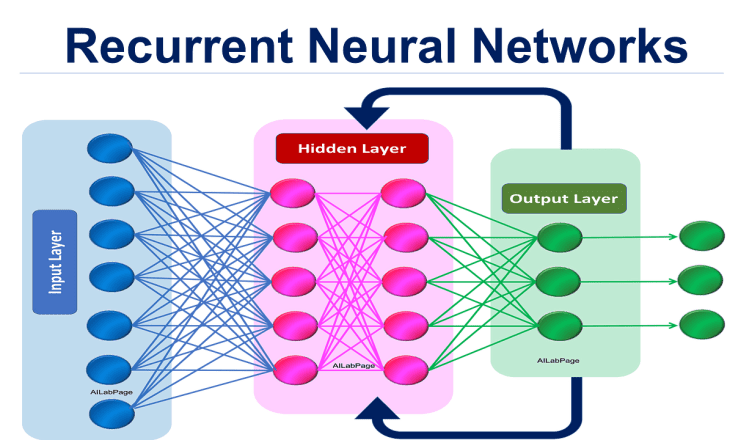
\includegraphics[width=\linewidth]{bibliography/rnn_fig.png}
    \caption{Model of RNN}
    \label{fig7}
  \end{minipage}
\end{figure}

In RNN architectures, different time steps share the same weight, allowing the network to form cyclical connections over time. This weight sharing significantly reduces the temporal parameters in the RNN network system.

However, one limitation of RNNs is their capacity to retain only a limited number of steps from previous sequences, which makes them less effective for longer sequences. To address this limitation, Long Short-Term Memory (LSTM) networks were introduced, offering improved capabilities for handling longer sequences.
\subsection{ARIMA}
ARIMA models (Autoregressive Integrated Moving Average) were first introduced by George Box and Gwilym Jenkins in the early 1970s. They have since become a fundamental tool in time series analysis and forecasting. ARIMA model is commonly denoted as (p, d, q):
\begin{itemize}
  \item AR (Autoregressive): Auto-Regressive (AR): using a linear combination of past values of the variable. An autoregressive model of order \(\rho\) can be written:
  \[Y_t = \Phi_1 Y_{t-1} + \Phi_2 Y_{t-2} + ... + \Phi_p Y_{t-p} + \varepsilon_t\]
Where:
\begin{itemize}
  \item \( Y_t \) is the current value.
  \item \( \Phi_1, \Phi_2, \ldots, \Phi_p \) are model parameters.
  \item \( \varepsilon_t \) is the random error.
\end{itemize}
  \item I (Integrated): refers to the differentiation of the time series data.
  \item Moving Average (MA): uses past forecast errors in a regression-like model. “\(q\)” is the number of previous error values to consider for the forecast.
\[
Y_t = c + \varepsilon_t + \theta_1 \varepsilon_{t-1} + \theta_2 \varepsilon_{t-2} + \cdots + \theta_q \varepsilon_{t-q}
\]
Where:
\begin{itemize}
  \item \( Y_t \) is the current value.
  \item \( \varepsilon_t \) is the random error.
  \item \( \theta_1, \theta_2, \ldots, \theta_q \) are coefficients.
  \item \( c \) is a constant.
\end{itemize}
\end{itemize}
\subsection{LSTM}
The Long Short-Term Memory (LSTM) model represents a widely used variant of recurrent neural networks (RNNs). Specifically designed to address the challenge of long-term dependencies, LSTM is well-suited for processing and predicting time series data. This model employs a sophisticated gating mechanism to regulate the flow of information within memory cells. The gate structure includes input gates, forget gates, and output gates, each managed by sigmoid and tanh layers[8].
\begin{figure}[H]
  \centering
  \begin{minipage}{0.8\linewidth}
    \centering
    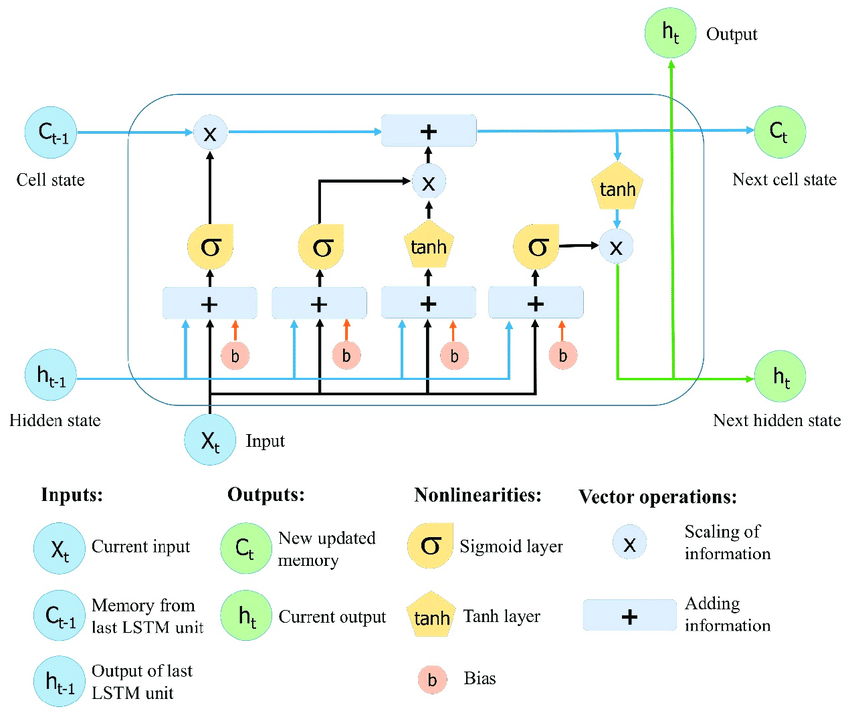
\includegraphics[width=\linewidth]{bibliography/lstm_fig.png}
    \caption{Model of LSTM}
    \label{fig8}
  \end{minipage}
\end{figure}
Schematic diagram of the LSTM neural network structure:
\begin{align}
\text{Sigmoid function:} & \quad \sigma(x) = \frac{1}{1 + e^{-x}} \tag{3} \\
\text{Tanh activation function:} & \quad \tanh(x) = \frac{e^x - e^{-x}}{e^x + e^{-x}} \notag \\
\text{Forget gate:} & \quad f_t = \sigma(W_f [h_{t-1}, x_t] + b_f) \tag{4} \\
\text{Input gate:} & \quad C_t = f_t \cdot C_{t-1} + i_t \cdot \hat{C}_t \tag{5} \\
& \quad \text{(Where the calculation methods of }\notag \\
& \quad i_t \text{ and } \hat{C}_t \text{ are shown in Eqs. 4 and 5)} \notag \\
\text{Output gate:} & \quad i_t = \sigma(W_i [h_{t-1}, x_t] + b_i) \tag{6} \\
& \quad \hat{C}_t = \tanh(W_c [h_{t-1}, x_t] + b_c) \tag{7} \\
& \quad o_t = \sigma(W_o [h_{t-1}, x_t] + b_o) \tag{8} \\
& \quad h_t = o_t \cdot \tanh(C_t) \tag{9}
\end{align}
Bi-LSTM: A bidirectional LSTM consists of two LSTM layers: a forward LSTM that processes the input sequence from start to end, and a backward LSTM that processes it from end to start. The outputs from both LSTMs are concatenated to produce the final output. By leveraging information from both past and future contexts, bidirectional LSTMs excel in tasks where understanding the entire context of the input sequence is crucial, such as natural language processing.
\begin{figure}[H]
  \centering
  \begin{minipage}{0.8\linewidth}
    \centering
    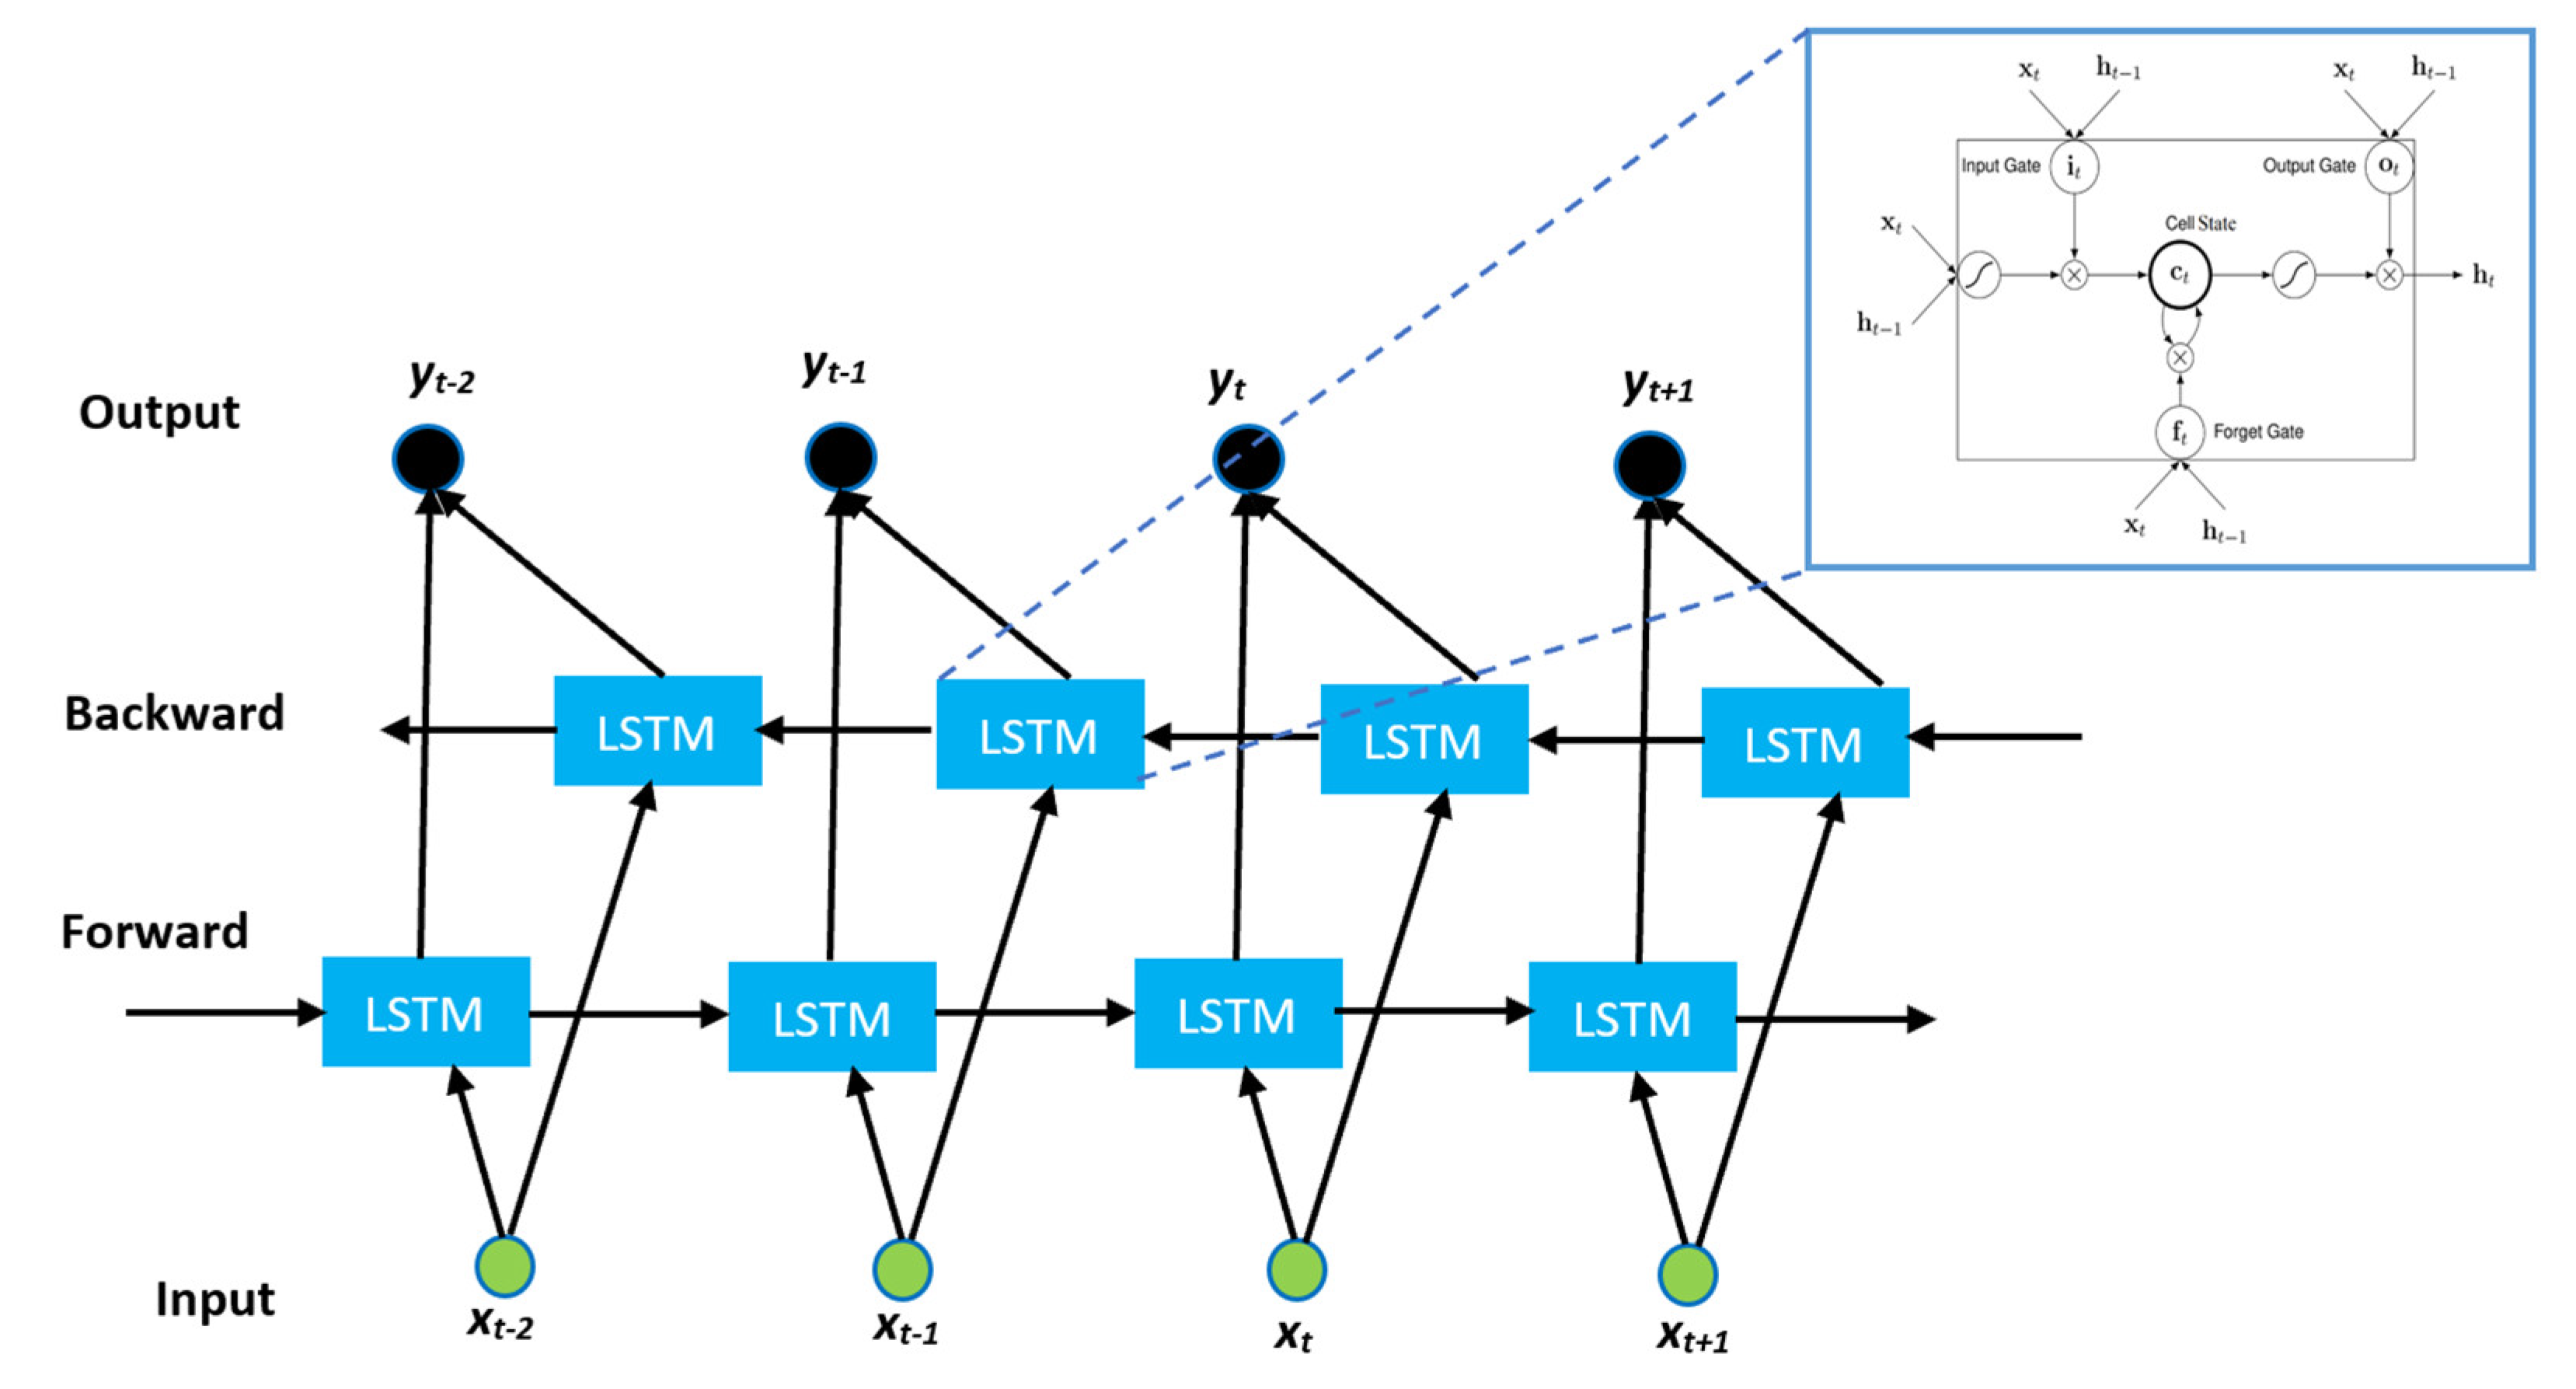
\includegraphics[width=\linewidth]{bibliography/bi-lstm_fig.png}
    \caption{Model of LSTM}
    \label{fig9}
  \end{minipage}
\end{figure}
\subsection{GRU}
	Gated Recurrent Unit (GRU) is a variant of the recurrent neural network (RNN) architecture, designed to improve the ability to store and process information in long-term data sequences without losing information. GRU uses gate mechanisms to selectively adjust the flow of information into and out of the hidden states of the network, allowing for efficient and selective updates of the state. The two main gates in GRU are the reset gate and the update gate.
\begin{figure}[H]
  \centering
  \begin{minipage}{0.8\linewidth}
    \centering
    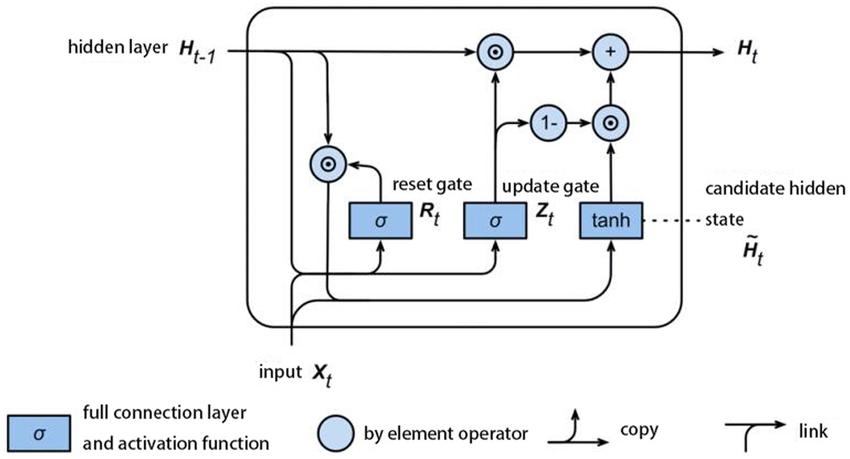
\includegraphics[width=\linewidth]{bibliography/gru_fig.png}
    \caption{Model of GRU}
    \label{fig10}
  \end{minipage}
\end{figure}
	\begin{itemize}
		\item Reset gate: Adjusts the amount of information from the previous hidden state that needs to be forgotten.
		\item Update gate: Decides the amount of new information from the input that will be used to update the hidden state.
	\end{itemize}
	GRU computes the output based on the updated hidden state through these gates, helping to maintain information effectively throughout the sequence processing.
	Below are the equations describing the GRU computation:
	   \begin{itemize}
    \item Reset gate:
    \begin{equation}
        r_t = \sigma(W_{xr} x_t + W_{hr} h_{t-1} + b_r)
    \end{equation}
    \item Update gate:
    \begin{equation}
        z_t = \sigma(W_{xz} x_t + W_{hz} h_{t-1} + b_z)
    \end{equation}
    \item Candidate hidden state:
    \begin{equation}
        \tilde{h}_t = \tanh(W_{xh} x_t + W_{hh} (r_t * h_{t-1}) + b_h)
    \end{equation}
    \item Final hidden state:
    \begin{equation}
        h_t = z_t * h_{t-1} + (1 - z_t) * \tilde{h}_t
    \end{equation}
        \end{itemize}
	Where:
	\begin{itemize}
		\item $W_{xr}, W_{xz}, W_{xh}$ are the learnable weight matrices.
		\item $x_t$ is the input at time step $t$.
		\item $h_{t-1}$ is the previous hidden state.
		\item $\sigma$ is the sigmoid activation function and $\tanh$ is the hyperbolic tangent activation function.
		\item $b_r, b_z, b_h$ are the bias terms.
	\end{itemize}
	By selectively adjusting the information flow through the gates, GRU can effectively handle long-term data sequences, especially useful in applications such as cryptocurrency price forecasting. GRU is simpler than LSTM but still maintains the powerful ability to process complex data sequences.
\subsection{GARCH}
The GARCH (Generalized AutoRegressive Conditional Heteroskedasticity) model is a statistical model that describes how the variance of error in a time series depends on past errors and variances. Unlike simple models that assume constant variance (homoskedasticity), GARCH allows for volatility, which means that periods of high and low volatility
can change based on historical data.
\\The general form of a GARCH(p, q) model is:
\[
\sigma^2_t = \omega + \alpha_1 \varepsilon^2_{t-1} + \alpha_2 \varepsilon^2_{t-2} + \cdots + \alpha_p \varepsilon^2_{t-p}
\]
\[
\quad + \beta_1 \sigma^2_{t-1} + \beta_2 \sigma^2_{t-2} + \cdots + \beta_q \sigma^2_{t-q}
\]

Where:
\begin{itemize}
  \item \(\sigma^2_t\) represents the conditional variance at time \(t\).
  \item \(\omega\) is the constant term or intercept.
  \item \(\alpha_1, \alpha_2, \ldots, \alpha_p\) are numeric coefficient for the squared residual for the past period.
  \item \(\beta_1, \beta_2, \ldots, \beta_q\) are numeric coefficient for the conditional variance from last period.
  \item \(\varepsilon^2_{t-1}, \varepsilon^2_{t-2}, \ldots, \varepsilon^2_{t-p}\) are squared residual for the past period.
  \item \(\sigma^2_{t-1}, \sigma^2_{t-2}, \ldots, \sigma^2_{t-q}\) are the past conditional variances.
\end{itemize}

In case GARCH(1:1), the formula will be:
\[
\sigma^2_t = \omega + \alpha_1 \varepsilon^2_{t-1} + \beta_1 \sigma^2_{t-1}
\]
\subsection{Gradient Boosting Regressor}

Gradient Boosting Regressor (GBR) is an ensemble machine learning technique that sequentially builds a series of weak learners, typically decision trees, to minimize a loss function and improve predictive accuracy.

Let \( \{ (x_i, y_i) \}_{i=1}^n \) be a training dataset where \( x_i \) represents the input features and \( y_i \) denotes the corresponding target values. GBR aims to approximate the target function \( F(x) \) by iteratively fitting additive models:

\[
F(x) = \sum_{m=1}^M \gamma_m h_m(x)
\]

where \( h_m(x) \) is the \( m \)-th weak learner (often a decision tree), and \( \gamma_m \) is the learning rate for the \( m \)-th iteration.

The GBR algorithm can be summarized as follows:

1. Initialize the model with a constant value, typically the mean of the target values \( \bar{y} = \frac{1}{n} \sum_{i=1}^n y_i \).
2. For \( m = 1 \) to \( M \):
   - Compute the negative gradient of the loss function with respect to the current model predictions \( -\frac{\partial L(y_i, F_{m-1}(x_i))}{\partial F_{m-1}(x_i)} \).
   - Fit a weak learner \( h_m(x) \) to predict the negative gradient residuals.
   - Determine the optimal step size \( \gamma_m \) using line search or another optimization method.
   - Update the model: \( F_m(x) = F_{m-1}(x) + \gamma_m h_m(x) \).

3. Continue iterating until a predefined number of iterations \( M \) is reached or until further iterations do not significantly improve performance.
\begin{figure}[H]
  \centering
  \begin{minipage}{0.8\linewidth}
    \centering
    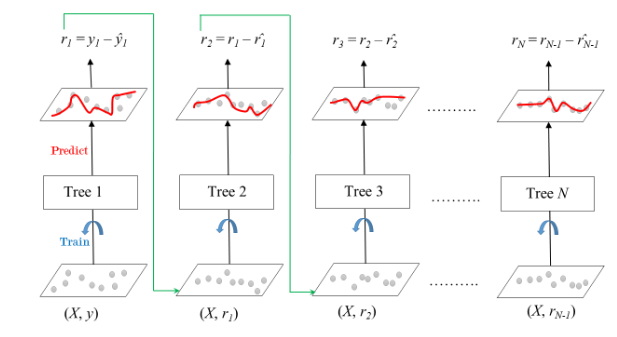
\includegraphics[width=\linewidth]{bibliography/gradientboosting_fig.png}
    \caption{Model of GBR}
    \label{fig11}
  \end{minipage}
\end{figure}
GBR combines the strengths of gradient descent optimization with boosting, effectively minimizing the error through an ensemble of weak learners. This method is particularly effective in scenarios where complex relationships exist between input features and target variables, making it widely used in predictive modeling across various domains.

\subsection{Multi-scale Isometric Convolution Network}
\subsubsection{MICN Model}
The Multi-scale Isometric Convolution Network (MICN), presented by Wang et al. in 2022, represents a significant advancement in long-term series forecasting. This model integrates multi-scale local and global context modeling techniques to effectively capture complex patterns and dependencies within time-series data.
\subsubsection{MICN Framework}
MICN Framework Overview: The MICN framework aims to predict a future time series of length \( O \) based on a historical series of length \( I \). It incorporates multi-scale hybrid decomposition (MHDecomp) blocks to separate complex patterns in the input series. It uses Seasonal Prediction Blocks to forecast seasonal information and Trend-cyclical Prediction Blocks to predict trend-cyclical patterns. The final prediction \( Y_{pred} \) is obtained by aggregating these prediction results. Here, \( d \) represents the number of variables in the multivariate time series, and \( D \) denotes the hidden state of the series.

\begin{figure}[H]
  \centering
  \begin{minipage}{1\linewidth}
    \centering
    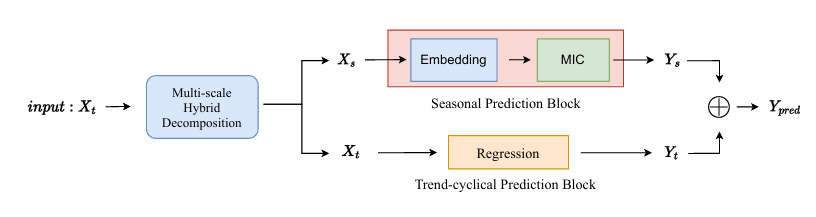
\includegraphics[width=\linewidth]{bibliography/micn_fig.png}
    \caption{Model of MICN}
    \label{fig11}
  \end{minipage}
\end{figure}

For the input series \( X \in \mathbb{R}^{I \times d} \):

\textbf{Trend-Cyclical Prediction Block:} MICN employs a linear regression strategy within the Trend-Cyclical Prediction Block to forecast the trend component of the time series. This method contrasts with simpler averaging techniques used in previous models, demonstrating improved forecasting accuracy for non-stationary series.

\[ Y_{\text{t}}^{regre} = \text{regression}(X_t) \]

where \( Y_{\text{t}}^{regre} \in \mathbb{R}^{O \times d} \) denotes the prediction of the trend part using the linear regression strategy.

\textbf{Seasonal Prediction Block:} The Seasonal Prediction Block focuses on modeling complex seasonal variations using multi-scale isometric convolution. It embeds input sequences to capture local features and global correlations across different scales, enhancing the model's capability to handle seasonal patterns robustly.

\begin{figure}[H]
  \centering
  \begin{minipage}{1\linewidth}
    \centering
    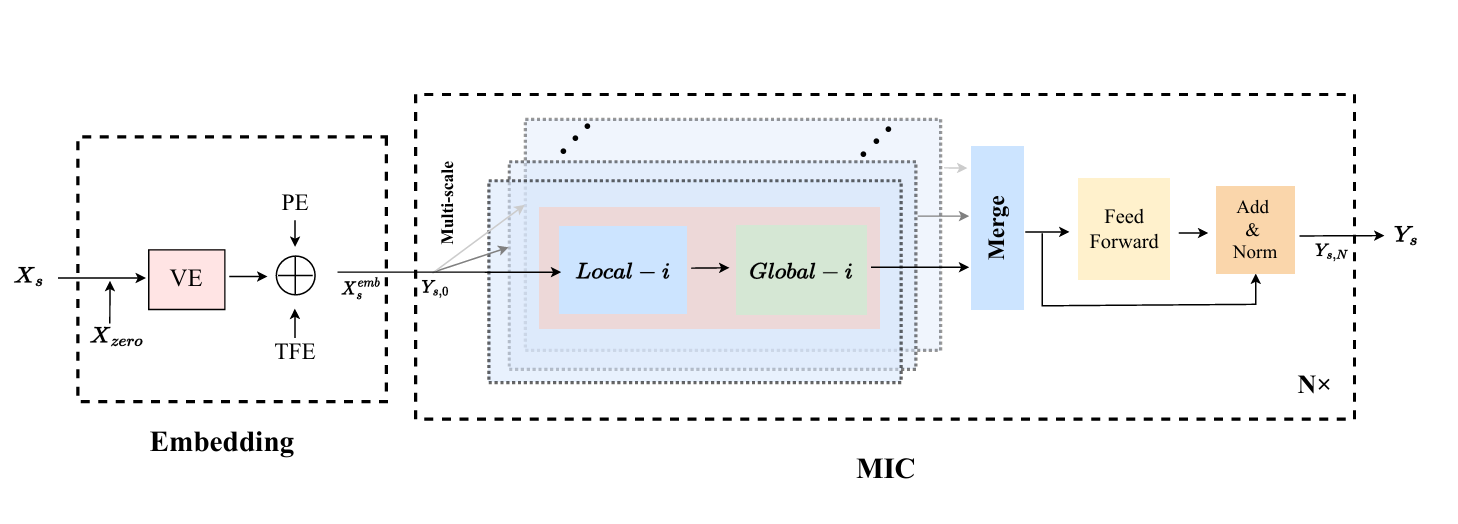
\includegraphics[width=\linewidth]{bibliography/micn_fig2.png}
    \caption{Model of MICN}
    \label{fig11}
  \end{minipage}
\end{figure}

\subsubsection{Methodologies}

\textbf{Multi-scale Isometric Convolution:} MICN utilizes multi-scale isometric convolution to capture both local and global dependencies within time-series data. This technique allows the model to extract comprehensive information from input sequences and improve forecasting accuracy.

\noindent \textbf{Embedding Layer:} The embedding layer in MICN integrates time features encoding, positional encoding, and value embedding to represent input sequences effectively. This approach minimizes redundant calculations and adapts well to varying prediction lengths \( O \).

\section{Result}
\subsection{Evaluation Methods}
\textbf{Mean Percentage Absolute Error} (MAPE): is a metric for evaluating the accuracy of a forecasting model. It measures the average magnitude of errors between predicted and actual values, expressed as a percentage. MAPE is defined as:\\
\[
\text{MAPE} = \frac{1}{n} \sum_{t=1}^{n} \left| \frac{y_t - \hat{y}_t}{y_t} \right| \times 100
\]

where:
\begin{itemize}
    \item \( n \) is the number of observations.
    \item \( y_t \) is the actual value at time \( t \).
    \item \( \hat{y}_t \) is the predicted value at time \( t \).
\end{itemize}
\textbf{Root Mean Squared Error} (RMSE): measures the square root of the average of the squared differences between the predicted and actual values. It is defined as:\\
\[
\text{RMSE} = \sqrt{\frac{1}{n} \sum_{t=1}^{n} (y_t - \hat{y}_t)^2}
\]

where:
\begin{itemize}
    \item \( n \) is the number of observations.
    \item \( y_t \) is the actual value at time \( t \).
    \item \( \hat{y}_t \) is the predicted value at time \( t \).
\end{itemize}
\textbf{Mean Absolute Error} (MAE): measures the average magnitude of the errors between predicted and actual values without considering their direction. MAE is defined as:\\

\[
\text{MAE} = \frac{1}{n} \sum_{t=1}^{n} \left| y_t - \hat{y}_t \right|
\]

where:
\begin{itemize}
    \item \( n \) is the number of observations.
    \item \( y_t \) is the actual value at time \( t \).
    \item \( \hat{y}_t \) is the predicted value at time \( t \).
\end{itemize}

\subsection{VCB Dataset} 
\begin{table}[H]
    \centering
    \begin{tabular}{|c|c|c|c|c|}
         \hline
         \multicolumn{5}{|c|}{\textbf{VCB Dataset's Evaluation}}\\
         \hline
         \centering Model & Training:Testing & MAPE (\%) & RMSE & MAE\\
         \hline
         \multirow{2}{*}{LN} & 7:3 & 9.8 & 9308.642 & 8307.594 \\ & 8:2 & 11.6 & 10929.857 & 10378.652 \\ & \textbf{9:1} & \textbf{6.9} & \textbf{7141.888} & \textbf{6311.754}\\
         \hline
         \multirow{2}{*}{ARIMA} & 7:3&1.04&1175.745&848.698\\ & 8:2&0.92&1128.364&813.264 \\ & \textbf{9:1} & \textbf{0.807} & \textbf{1053.277} & \textbf{728.787}\\
         \hline
         \multirow{2}{*}{RNN} & 7:3 & 2.756 & 84912.220 & 84743.142 \\ 
& 8:2 & 2.768 & 87906.756 & 87839.897 \\ 
& \textbf{9:1} & \textbf{1.676} & \textbf{92428.848} & \textbf{92400.334} \\
         \hline
         \multirow{2}{*}{LSTM} & 7:3 &  1.83 &  2064.552 & 1601.095 \\ & 8:2 &  2.13 & 2328.359 & 1922.049 \\ & \textbf{9:1} &\textbf{1.54}  & \textbf{2122.498} &\textbf{1455.057}\\
         \hline
         \multirow{2}{*}{GRU} & 7:3 & 1.04 & 1240.390 & 911.386 \\ & 8:2 & 0.99 & 1231.421 & 889.385 \\ & \textbf{9:1} & \textbf{0.6} & \textbf{798.720} & \textbf{614.843}\\
         \hline
         \multirow{2}{*}{GARCH} & 7:3 & nan & 2.097 & 1.741 \\ 
            & 8:2 & nan & 1.950 & 1.661 \\
            & \textbf{9:1} & \textbf{nan} & \textbf{1.865} & \textbf{1.617} \\
         \hline
       \multirow{2}{*}{GBR} & 7:3 & 8.6 & 9507.772 & 7663.113 \\ 
            & 8:2 & 9.3 & 9202.547 & 8350.244 \\ 
            & \textbf{9:1} & \textbf{1.9} & \textbf{2230.027} & \textbf{1748.122} \\
         \hline
        \multirow{2}{*}{MICN} & 7:3 & 19.0 & 18350.763 & 16502.455 \\ 
            & 8:2 & 22.2 & 20136.471 & 19749.414 \\ 
            & \textbf{9:1} & \textbf{16.6} & \textbf{15341.417} & \textbf{15027.681} \\
         \hline
    \end{tabular}
    \caption{VCB Dataset's Evaluation}
    \label{vcbresult}
\end{table}


\begin{figure}[H]
  \centering
  \begin{minipage}{0.8\linewidth}
    \centering
    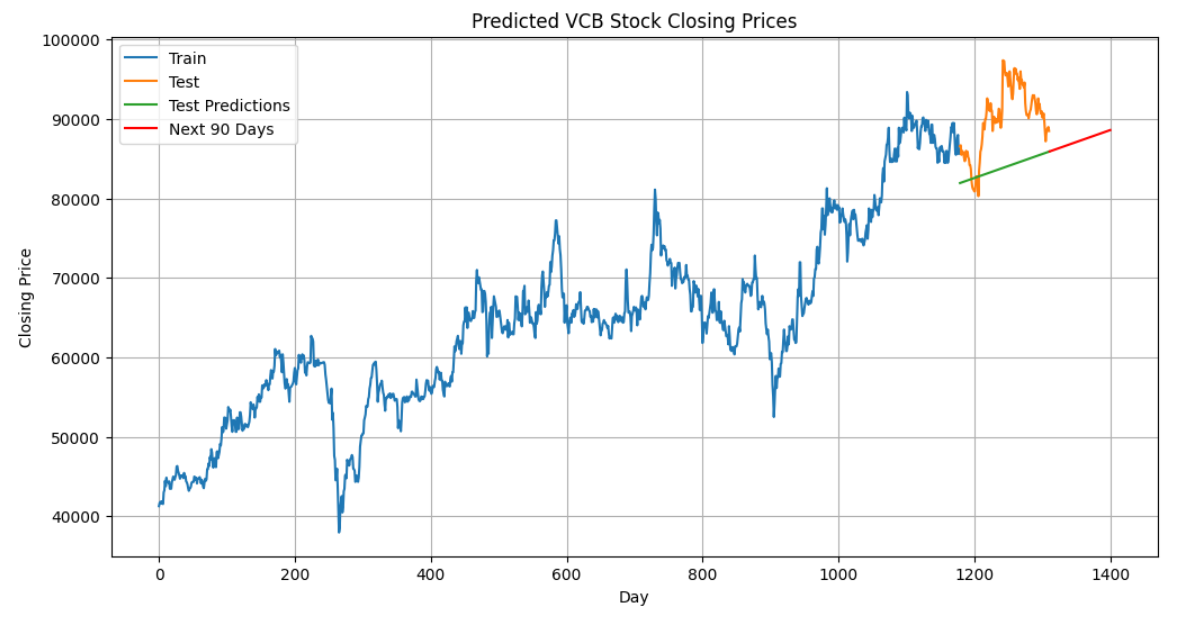
\includegraphics[width=\linewidth]{bibliography/VCB-LN-9-1.png}
    \caption{LN model's result with 9:1 splitting proportion}
    \label{fig8}
  \end{minipage}
\end{figure}
\begin{figure}[H]
  \centering
  \begin{minipage}{0.8\linewidth}
    \centering
    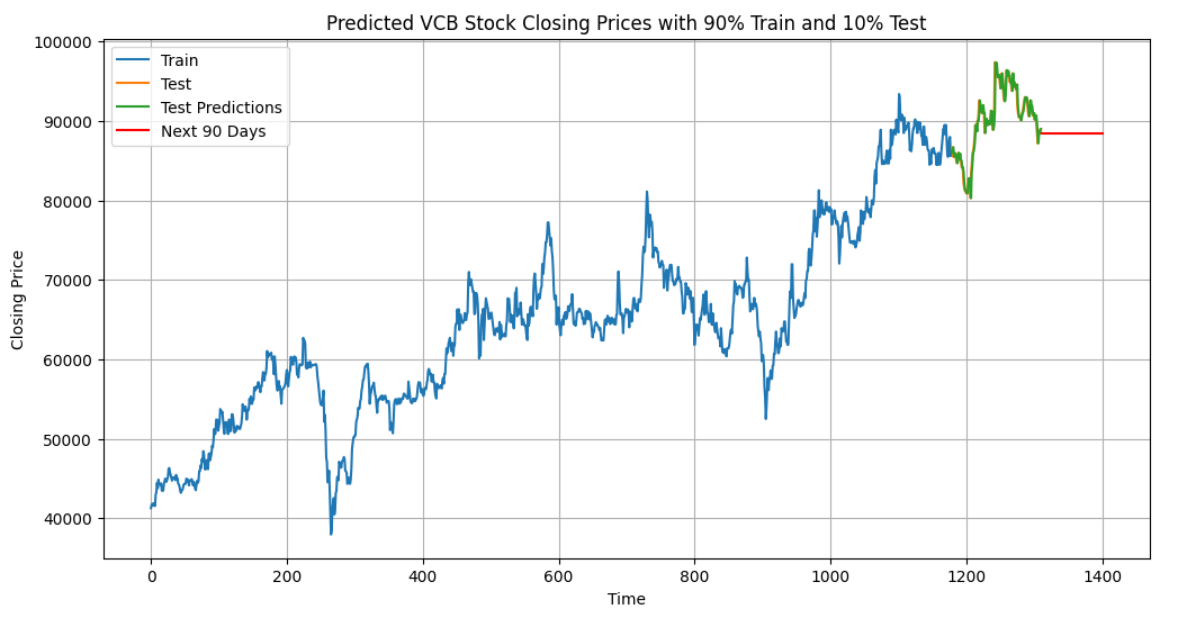
\includegraphics[width=\linewidth]{bibliography/VCB-ARIMA-9-1.png}
    \caption{ARIMA model's result with 9:1 splitting proportion}
    \label{fig8}
  \end{minipage}
\end{figure}
\begin{figure}[H]
  \centering
  \begin{minipage}{0.8\linewidth}
    \centering
    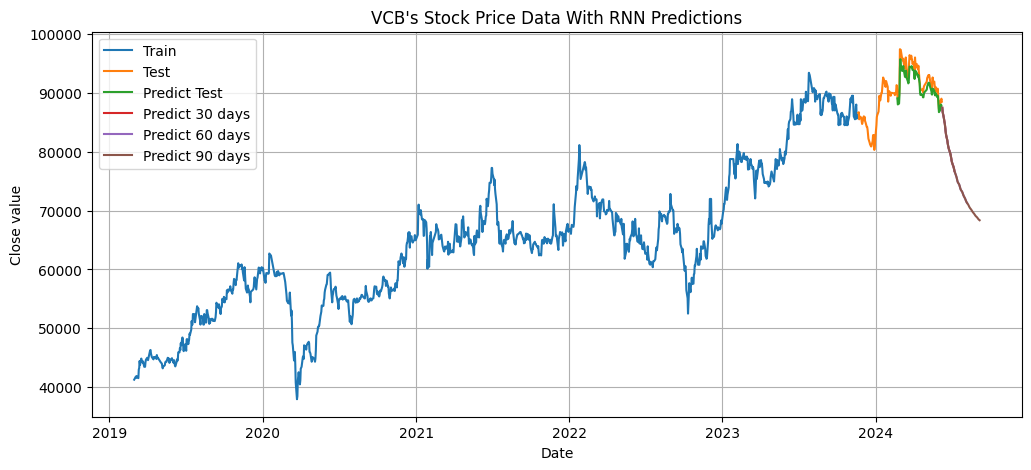
\includegraphics[width=\linewidth]{bibliography/VCB-RNN-9-1.png}
    \caption{RNN model's result with 9:1 splitting proportion}
    \label{fig8}
  \end{minipage}
\end{figure}
\begin{figure}[H]
  \centering
  \begin{minipage}{0.8\linewidth}
    \centering
    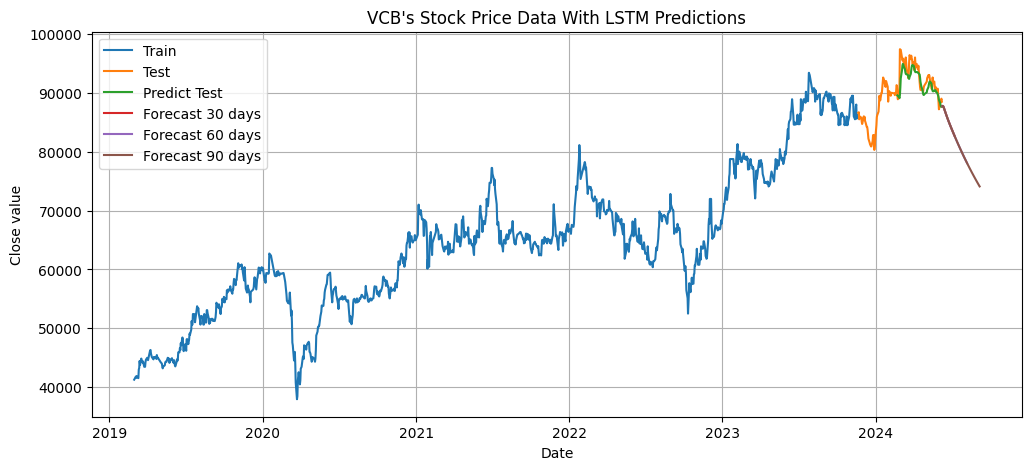
\includegraphics[width=\linewidth]{bibliography/VCB-LSTM-9-1.png}
    \caption{LSTM model's result with 9:1 splitting proportion}
    \label{fig9}
  \end{minipage}
\end{figure}
\begin{figure}[H]
  \centering
  \begin{minipage}{0.8\linewidth}
    \centering
    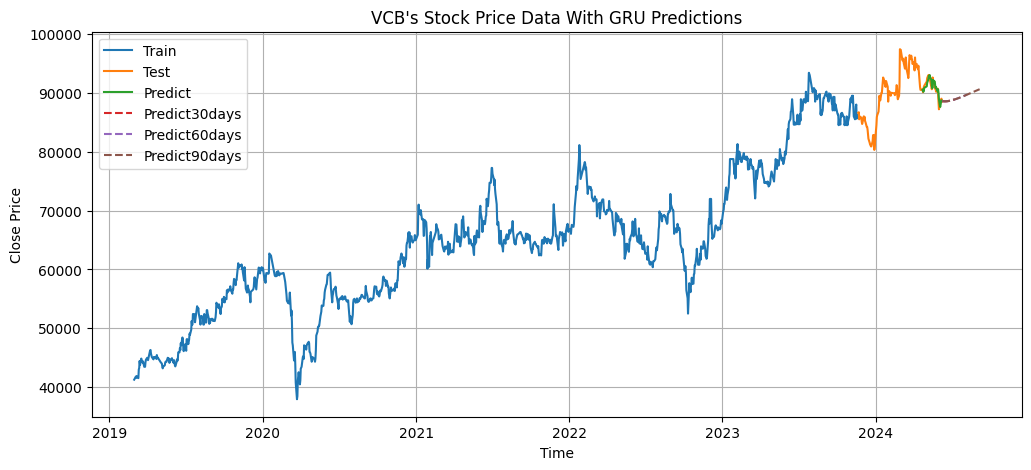
\includegraphics[width=\linewidth]{bibliography/VCB-GRU-9-1.png}
    \caption{GRU model's result with 9:1 splitting proportion}
    \label{fig10}
  \end{minipage}
\end{figure}
\begin{figure}[H]
  \centering
  \begin{minipage}{0.8\linewidth}
    \centering
    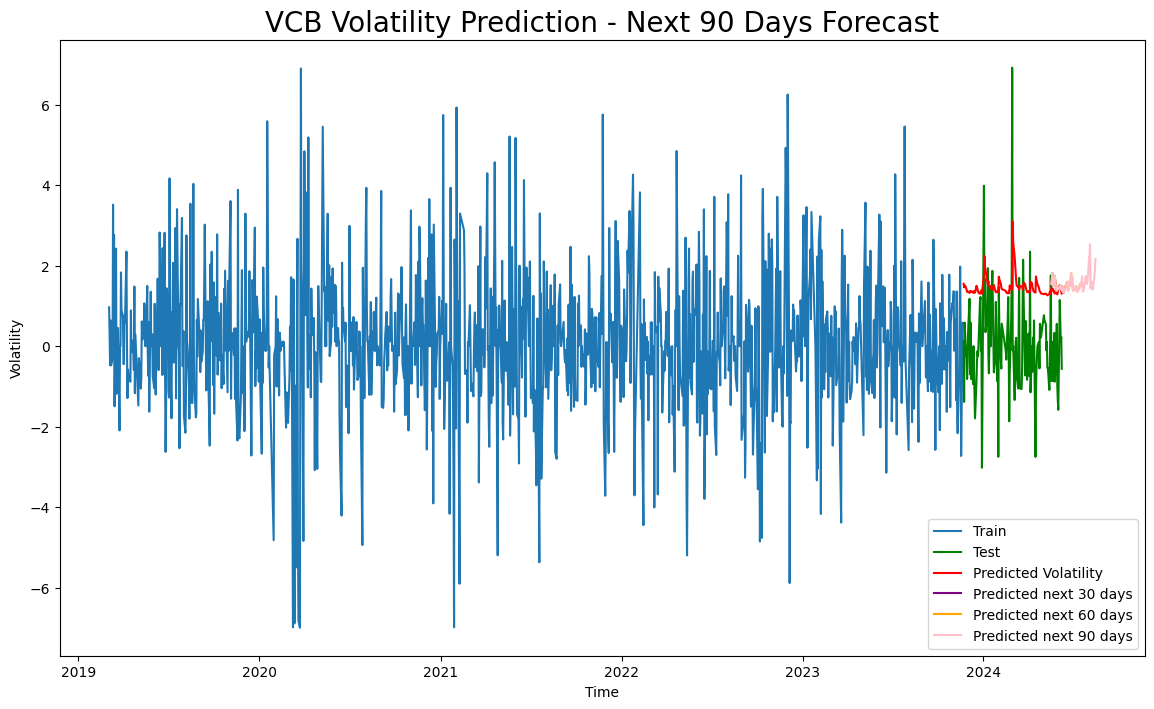
\includegraphics[width=\linewidth]{bibliography/VCB-GARCH-9-1.png}
    \caption{GARCH model's result with 9:1 splitting proportion}
    \label{fig11}
  \end{minipage}
\end{figure}
\begin{figure}[H]
  \centering
  \begin{minipage}{0.8\linewidth}
    \centering
    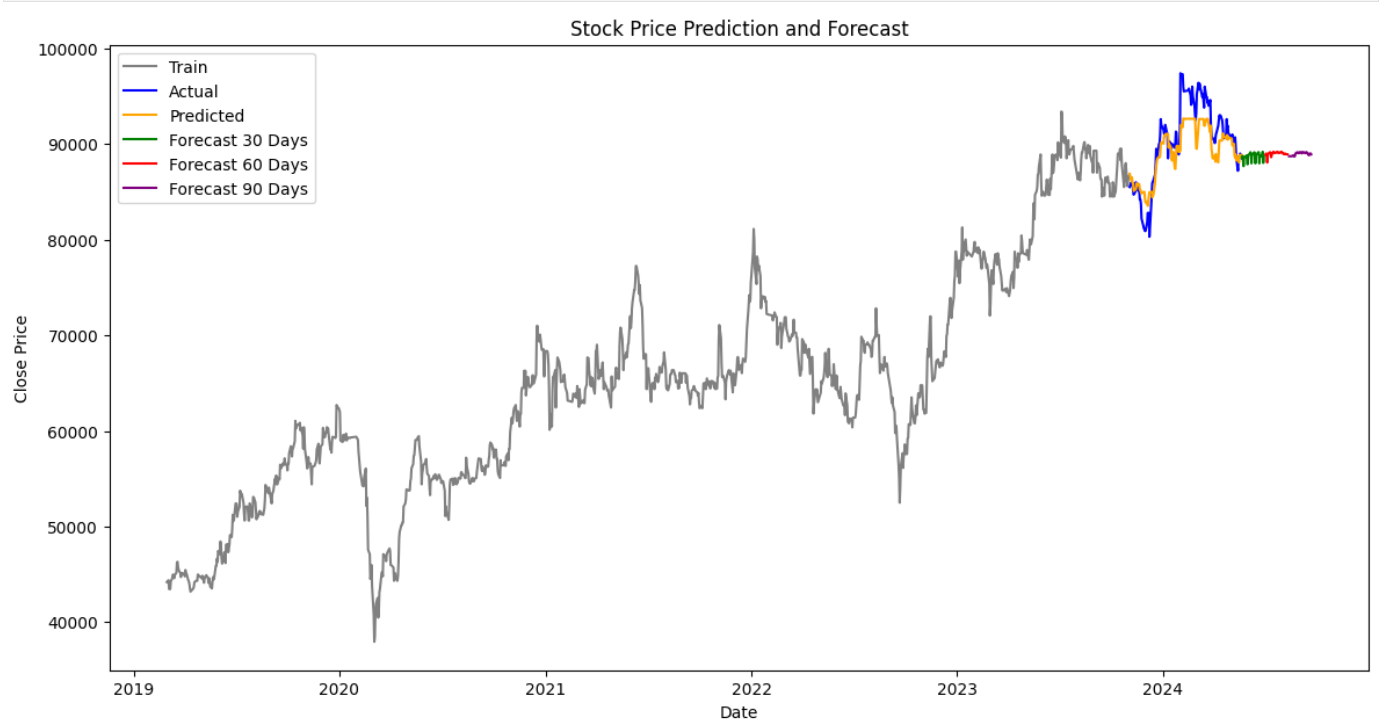
\includegraphics[width=\linewidth]{bibliography/VCB-GBR-9-1.png}
    \caption{GBR model's result with 9:1 splitting proportion}
    \label{fig12}
  \end{minipage}
\end{figure}
\begin{figure}[H]
  \centering
  \begin{minipage}{0.8\linewidth}
    \centering
    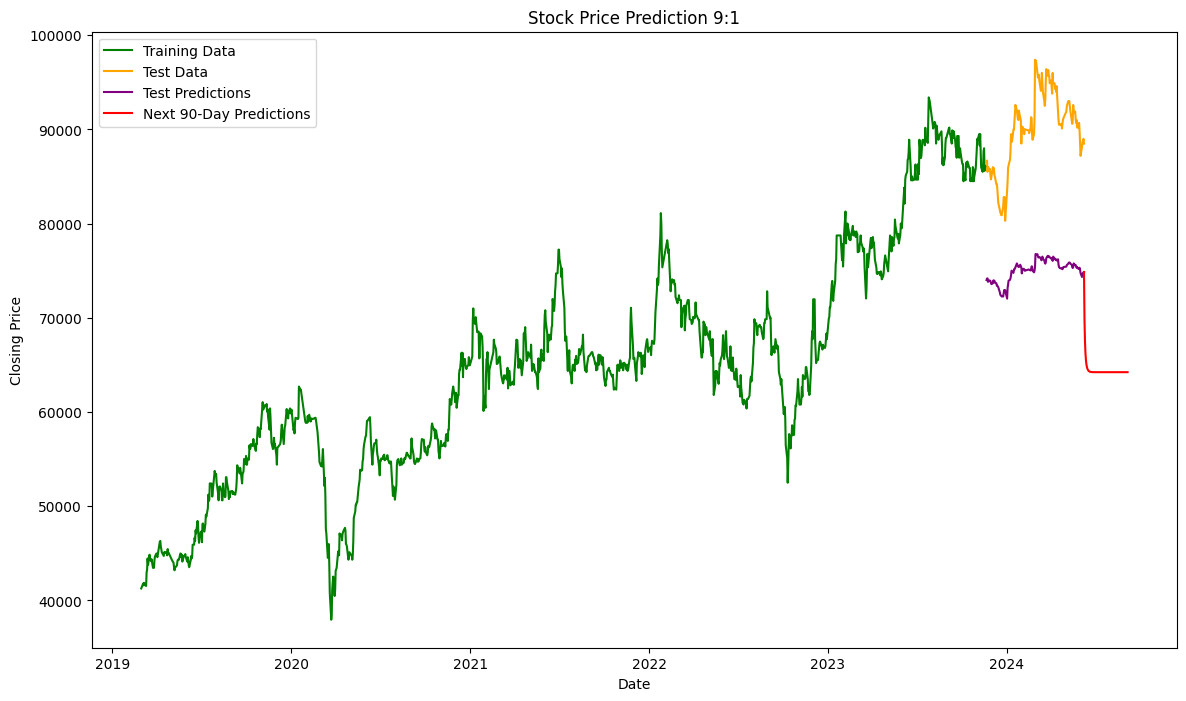
\includegraphics[width=\linewidth]{bibliography/VCB-MICN-9-1.png}
    \caption{MICN model's result with 9:1 splitting proportion}
    \label{fig13}
  \end{minipage}
\end{figure}

\subsection{ACB dataset} 
\begin{table}[H]
    \centering
    \begin{tabular}{|c|c|c|c|c|}
         \hline
         \multicolumn{5}{|c|}{\textbf{ACB Dataset's Evaluation}}\\
         \hline
         \centering Model & Training:Testing & MAPE (\%) & RMSE & MAE\\
         \hline
         \multirow{2}{*}{LN} & 7:3 & 24.1 & 4812.948 & 4679.671 \\ 
         & 8:2 & 11.7 & 2682.869 & 2320.709 \\ 
         & \textbf{9:1} & \textbf{5.3} & \textbf{1454.617} & \textbf{1158.013}\\
         \hline
         \multirow{2}{*}{ARIMA} & 7:3 & 1.06 & 294.170 & 208.677 \\ 
         & \textbf{8:2} & \textbf{0.90} & \textbf{274.825} & \textbf{192.154} \\ 
         & 9:1 & 0.95 & 308.451 & 218.907 \\
         \hline
         \multirow{2}{*}{RNN} & \textbf{7:3} & \textbf{2.01} & \textbf{20638.496} & \textbf{20543.834} \\ 
         &  8:2 & 2.37 & 21701.767 & 21614.888 \\ 
         & 9:1 & 3.03 & 23590.512 & 23585.406 \\
         \hline
         \multirow{2}{*}{LSTM} & 7:3 & 3.23 & 917.183 & 705.928 \\ 
         & \textbf{8:2} & \textbf{2.39} & \textbf{666.151} & \textbf{531.216} \\ 
         & 9:1 & 3.45 & 963.564 & 840.762 \\
         \hline
         \multirow{2}{*}{GRU} & \textbf{7:3} & \textbf{1.02} & \textbf{307.166} & \textbf{218.966} \\ 
         & 8:2 & 1.37 & 409.880 & 310.602 \\ 
         & 9:1 & 1.23 & 388.034 & 301.499 \\
         \hline
         \multirow{2}{*}{GARCH} & 7:3 & nan & 2.171 & 1.718 \\ 
         & \textbf{8:2} & \textbf{nan} & \textbf{1.832} & \textbf{1.514} \\
         & 9:1 & nan & 1.848 & 1.518 \\
         \hline
         \multirow{2}{*}{GBR} & \textbf{7:3} & \textbf{3.6} & \textbf{1418.069} & \textbf{819.109} \\ 
         & 8:2 & 4.6 & 1677.833 & 1086.011 \\ 
         & 9:1 & 7.8 & 2260.802 & 1865.096 \\
         \hline
         \multirow{2}{*}{MICN} & \textbf{7:3} & \textbf{6.6} & \textbf{2186.285} & \textbf{1438.314} \\ 
         & 8:2 & 15.1 & 3922.045 & 3363.858 \\ 
         & 9:1 & 19.3 & 4786.054 & 4513.602 \\
         \hline
    \end{tabular}
    \caption{ACB Dataset's Evaluation}
    \label{acbresult}
\end{table}
\begin{figure}[H]
  \centering
  \begin{minipage}{0.8\linewidth}
    \centering
    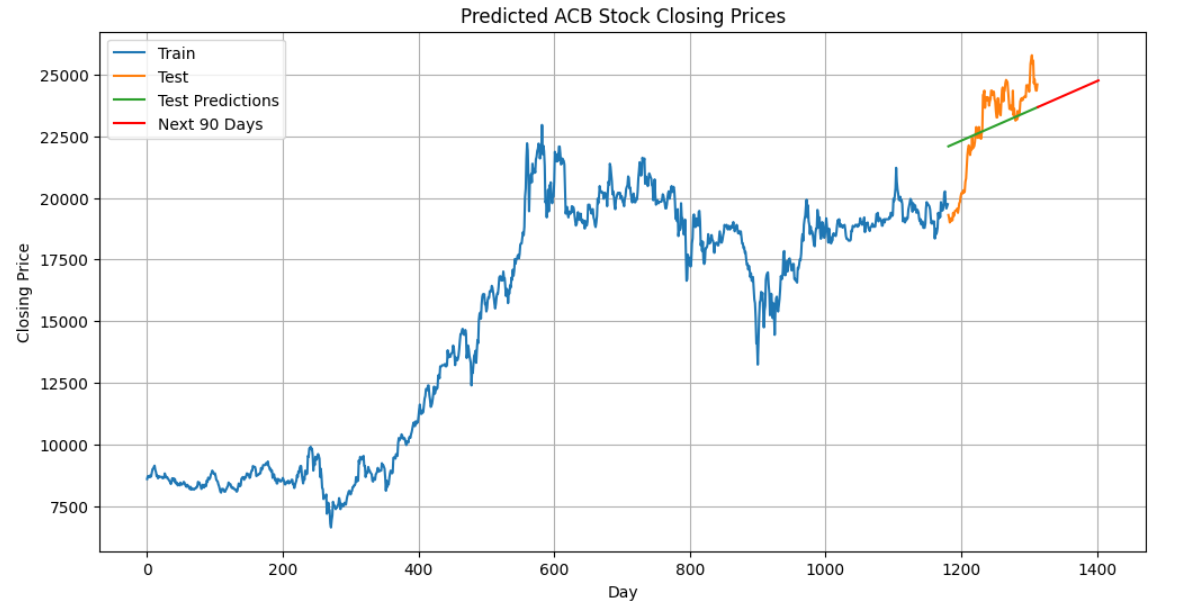
\includegraphics[width=\linewidth]{bibliography/ACB-LN-9-1.png}
    \caption{LN model's result with 9:1 splitting proportion}
    \label{fig15}
  \end{minipage}
\end{figure}
\begin{figure}[H]
  \centering
  \begin{minipage}{0.8\linewidth}
    \centering
    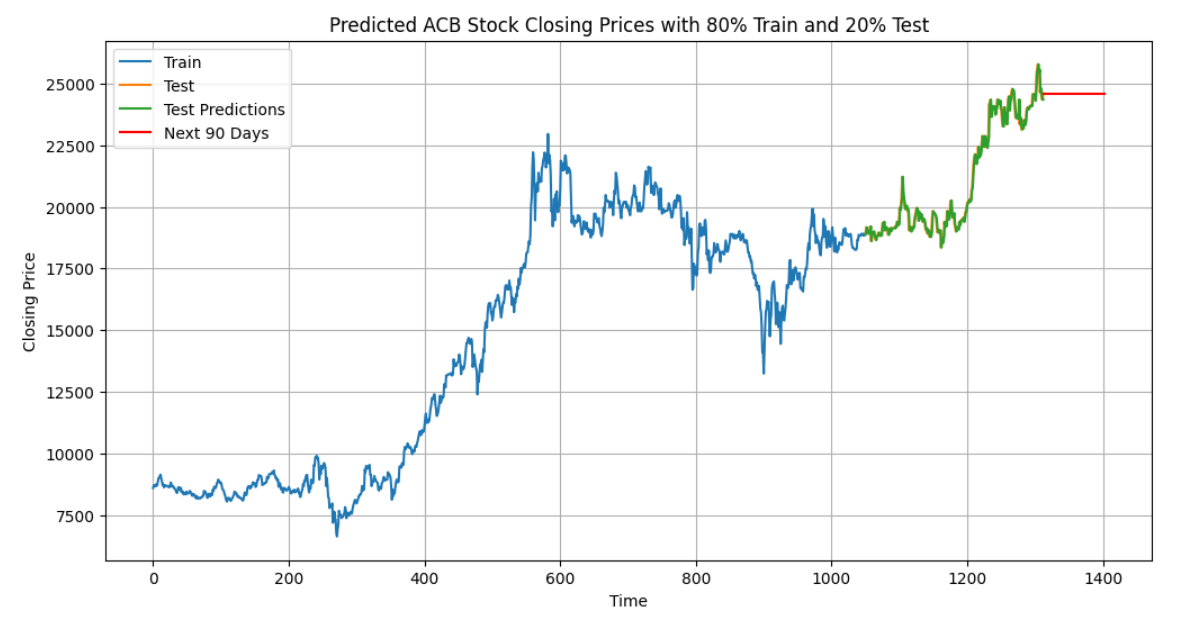
\includegraphics[width=\linewidth]{bibliography/ACB-ARIMA-8-2.png}
    \caption{ARIMA model's result with 8:2 splitting proportion}
    \label{fig16}
  \end{minipage}
\end{figure}
\begin{figure}[H]
  \centering
  \begin{minipage}{0.8\linewidth}
    \centering
    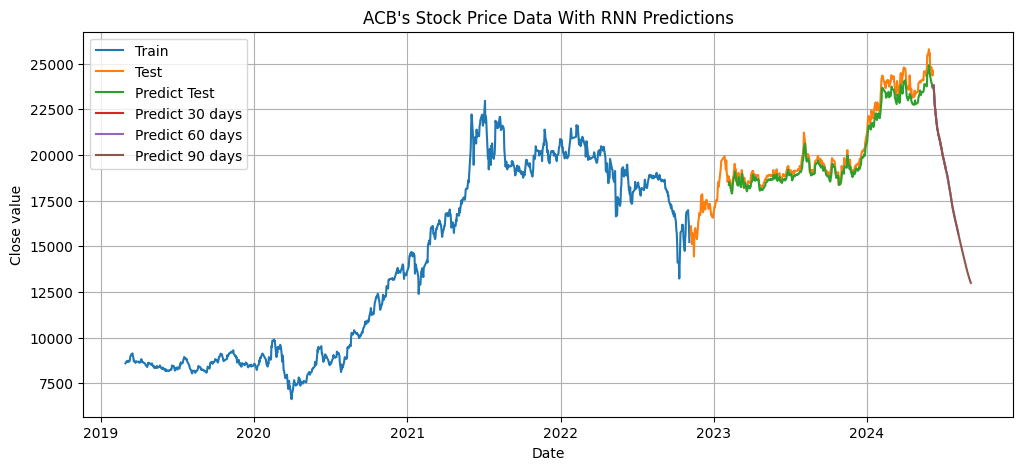
\includegraphics[width=\linewidth]{bibliography/ACB-RNN-7-3.png}
    \caption{RNN model's result with 7:3 splitting proportion}
    \label{fig17}
  \end{minipage}
\end{figure}
\begin{figure}[H]
  \centering
  \begin{minipage}{0.8\linewidth}
    \centering
    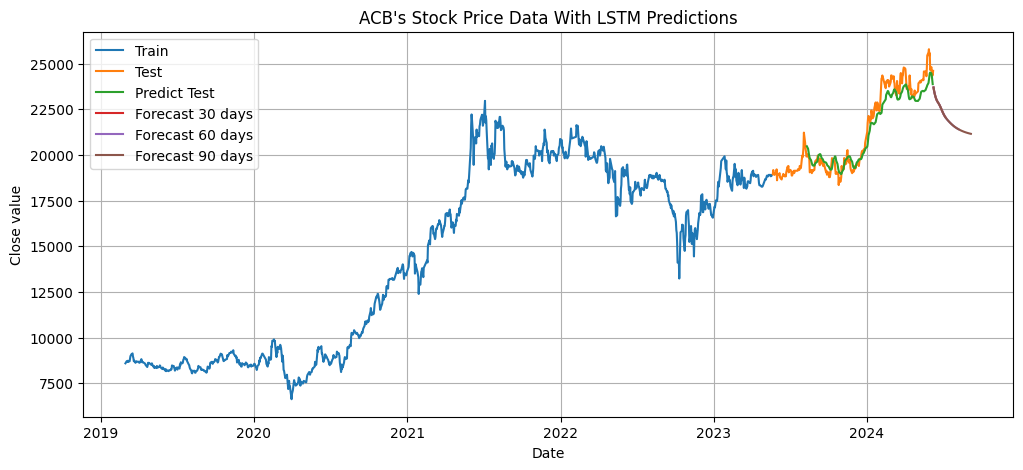
\includegraphics[width=\linewidth]{bibliography/ACB-LSTM-8-2.png}
    \caption{LSTM model's result with 9:1 splitting proportion}
    \label{fig18}
  \end{minipage}
\end{figure}
\begin{figure}[H]
  \centering
  \begin{minipage}{0.8\linewidth}
    \centering
    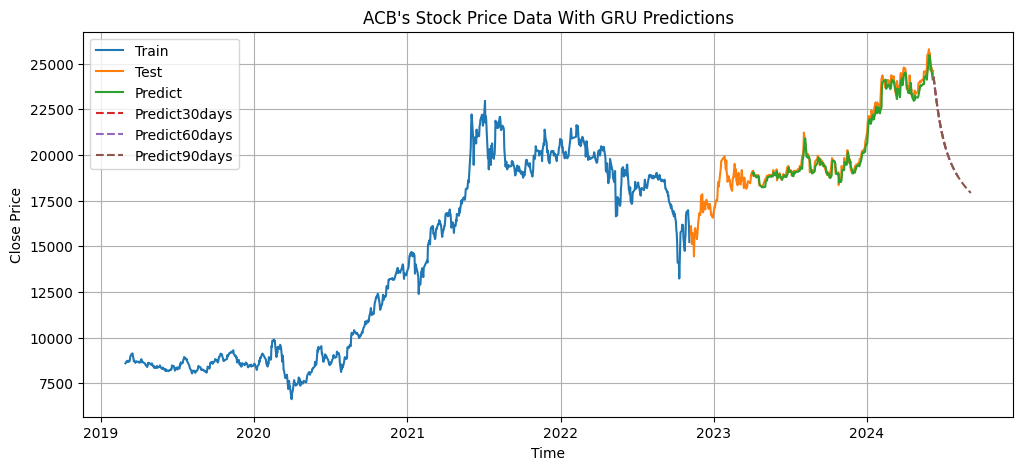
\includegraphics[width=\linewidth]{bibliography/ACB-GRU-7-3.png}
    \caption{GRU model's result with 7:3 splitting proportion}
    \label{fig8}
  \end{minipage}
\end{figure}
\begin{figure}[H]
  \centering
  \begin{minipage}{0.8\linewidth}
    \centering
    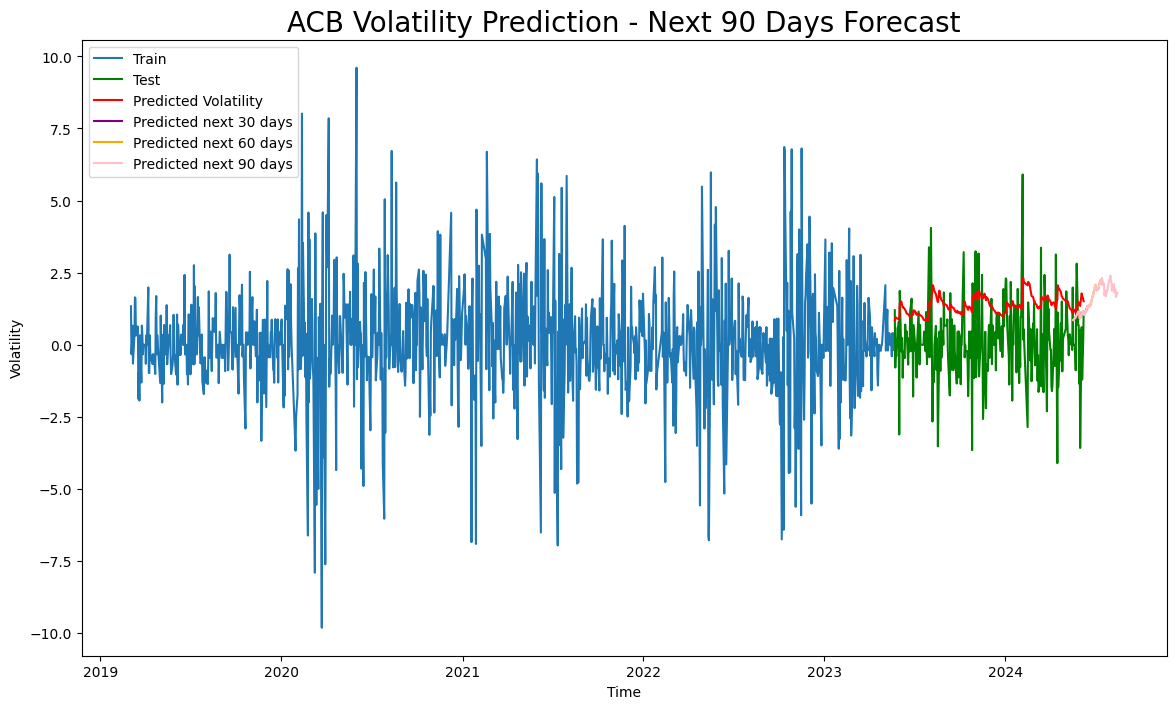
\includegraphics[width=\linewidth]{bibliography/ACB-GARCH-8-2.png}
    \caption{GARCH model's result with 8:2 splitting proportion}
    \label{fig8}
  \end{minipage}
\end{figure}
\begin{figure}[H]
  \centering
  \begin{minipage}{0.8\linewidth}
    \centering
    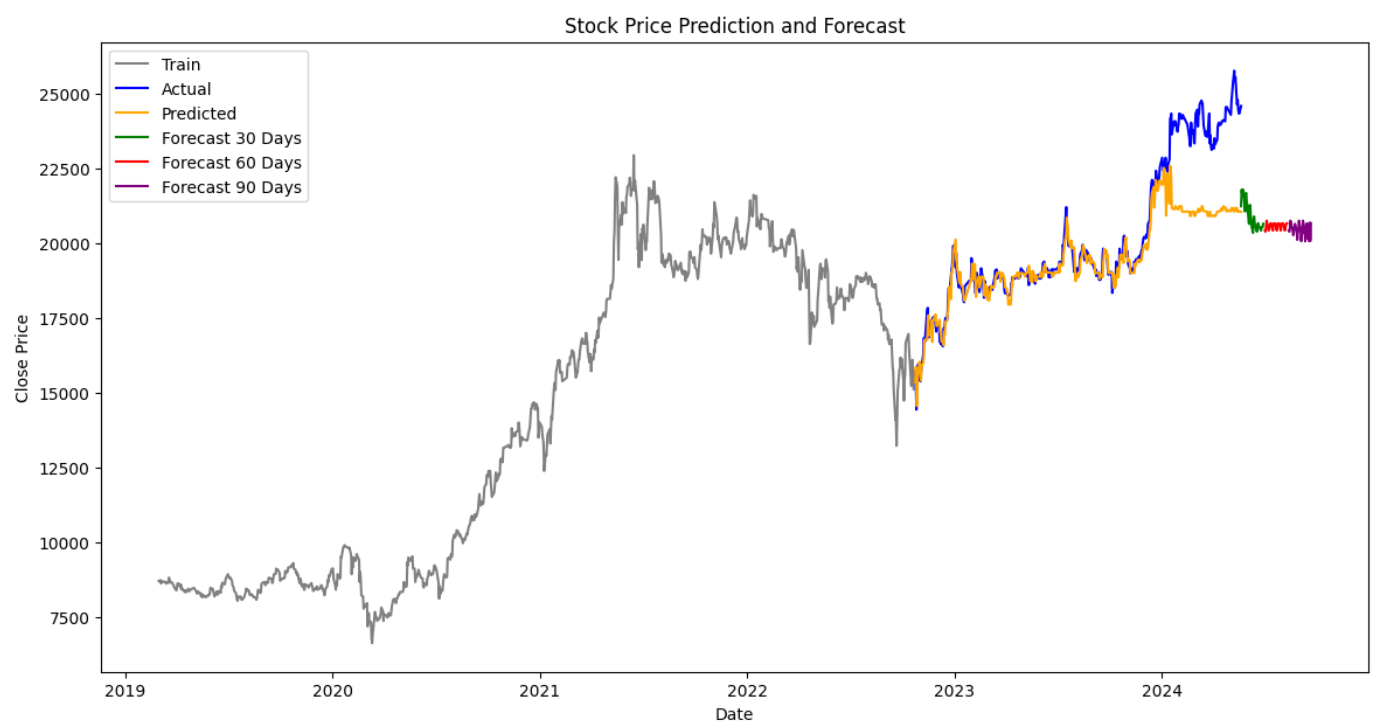
\includegraphics[width=\linewidth]{bibliography/ACB-GBR-7-3.png}
    \caption{GBR model's result with 7:3 splitting proportion}
    \label{fig18}
  \end{minipage}
\end{figure}
\begin{figure}[H]
  \centering
  \begin{minipage}{0.8\linewidth}
    \centering
    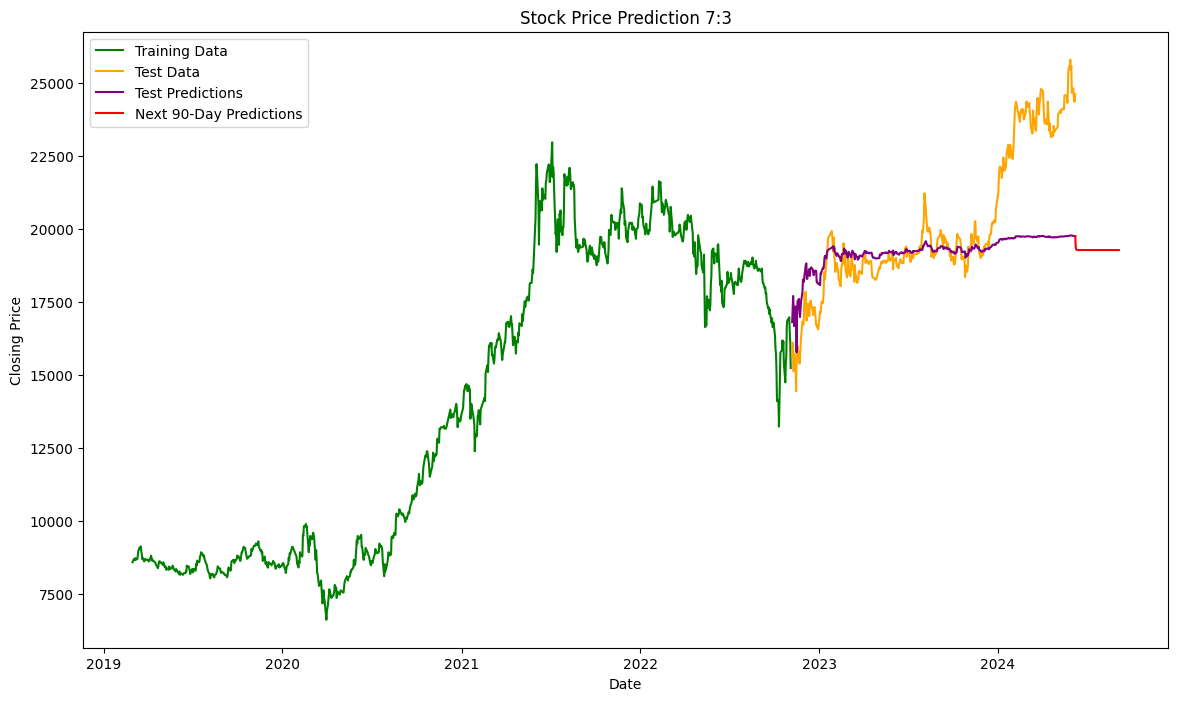
\includegraphics[width=\linewidth]{bibliography/ACB-MICN-7-3.png}
    \caption{MICN model's result with 7:3 splitting proportion}
    \label{fig19}
  \end{minipage}
\end{figure}

\subsection{CTG dataset} 
\begin{table}[H]
    \centering
    \begin{tabular}{|c|c|c|c|c|}
         \hline
         \multicolumn{5}{|c|}{\textbf{CTG Dataset's Evaluation}}\\
         \hline
         \centering Model & Training:Testing & MAPE (\%) & RMSE & MAE\\
         \hline
         \multirow{2}{*}{LN} & 7:3 & 23.5 & 6628.914 & 6240.569 \\ 
         & 8:2 & 11.8 & 3731.196 & 3233.027 \\ 
         & \textbf{9:1} & \textbf{8.4} & \textbf{3032.375} & \textbf{2643.229} \\
         \hline
         \multirow{2}{*}{ARIMA} & 7:3 & 1.336 & 523.846 & 371.441 \\ 
         & \textbf{8:2} & \textbf{1.187} & \textbf{521.978} & \textbf{356.312} \\ 
         & 9:1 & 1.294 & 610.492 & 422.452 \\
         \hline
         \multirow{2}{*}{RNN} & 7:3 & 2.465 & 28772.902 & 28581.666 \\ 
         & \textbf{8:2} & \textbf{2.353} & \textbf{30566.344} & \textbf{30365.371} \\ 
         & 9:1 & 2.568 & 33546.902 & 33520.913 \\
         \hline
         \multirow{2}{*}{LSTM} & 7:3 & 3.127 & 1141.069 & 924.030 \\ 
         & \textbf{8:2} & \textbf{2.304} & \textbf{936.059} & \textbf{713.297} \\ 
         & 9:1 & 3.542 & 1411.940 & 1207.337 \\
         \hline
         \multirow{2}{*}{GRU} & \textbf{7:3} & \textbf{1.236} & \textbf{508.833} & \textbf{363.608} \\ 
         & 8:2 & 1.360 & 595.657 & 427.719 \\ 
         & 9:1 & 1.344 & 574.250 & 440.853 \\
         \hline
         \multirow{2}{*}{GARCH} & 7:3 & nan & 2.641 & 2.088 \\ 
         & \textbf{8:2} & \textbf{nan} & \textbf{2.425} & \textbf{1.945} \\ 
         & 9:1 & nan & 2.594 & 2.059 \\
         \hline
         \multirow{2}{*}{GBR} & 7:3 & 1.6 & 615.558 & 441.555 \\ 
         & \textbf{8:2} & \textbf{1.4} & \textbf{626.922} & \textbf{432.788} \\ 
         & 9:1 & 1.7 & 781.218 & 568.495 \\
         \hline
         \multirow{2}{*}{MICN} & 7:3 & 9 & 3456.450 & 2711.102 \\ 
         & \textbf{8:2} & \textbf{5.7} & \textbf{2695.131} & \textbf{1861.530} \\ 
         & 9:1 & 12.5 & 4704.741 & 4176.037 \\
         \hline
    \end{tabular}
    \caption{CTG Dataset's Evaluation}
    \label{ctgresult}
\end{table}


\begin{figure}[H]
  \centering
  \begin{minipage}{0.8\linewidth}
    \centering
    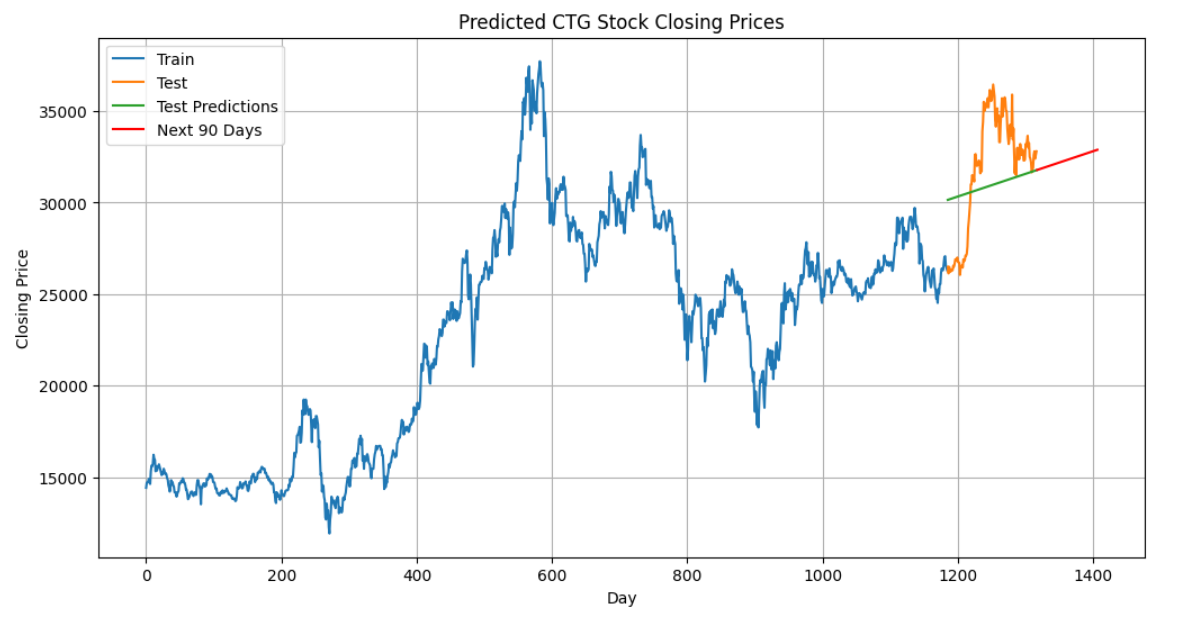
\includegraphics[width=\linewidth]{bibliography/CTG-LN-9-1.png}
    \caption{CTG model's result with 9:1 splitting proportion}
    \label{fig22}
  \end{minipage}
\end{figure}
\begin{figure}[H]
  \centering
  \begin{minipage}{0.8\linewidth}
    \centering
    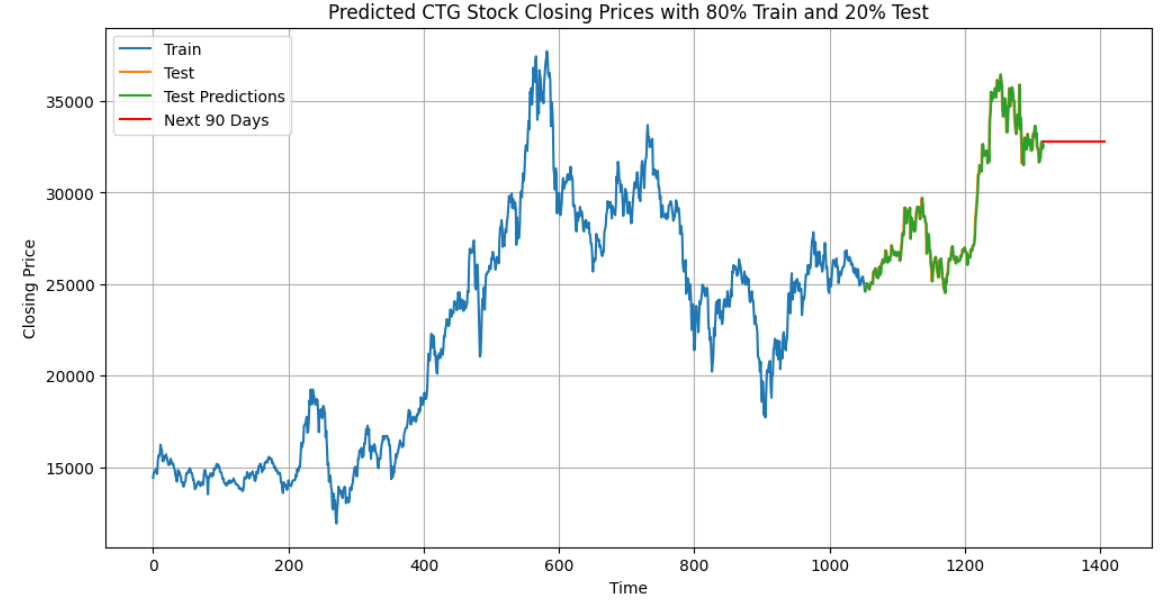
\includegraphics[width=\linewidth]{bibliography/CTG-ARIMA-8-2.png}
    \caption{ARIMA model's result with 8:2 splitting proportion}
    \label{fig23}
  \end{minipage}
\end{figure}
\begin{figure}[H]
  \centering
  \begin{minipage}{0.8\linewidth}
    \centering
    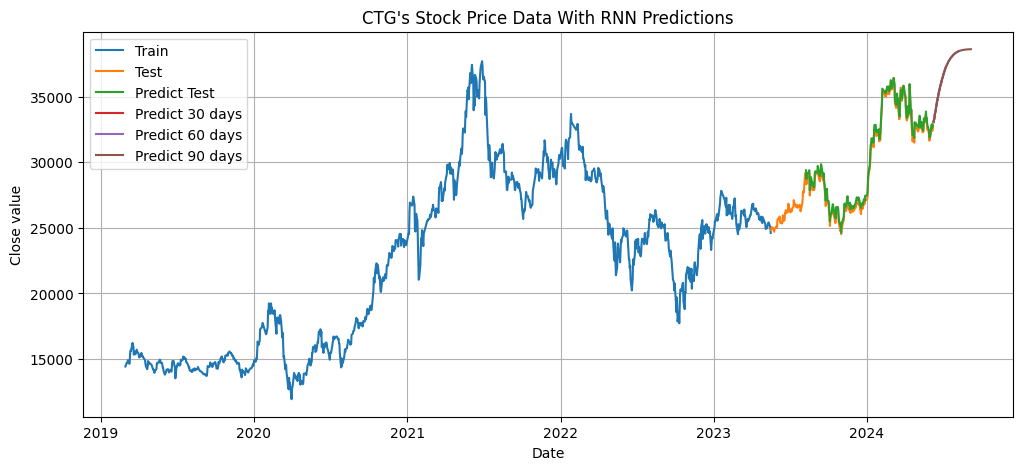
\includegraphics[width=\linewidth]{bibliography/CTG-RNN-8-2.png}
    \caption{RNN model's result with 8:2 splitting proportion}
    \label{fig24}
  \end{minipage}
\end{figure}
\begin{figure}[H]
  \centering
  \begin{minipage}{0.8\linewidth}
    \centering
    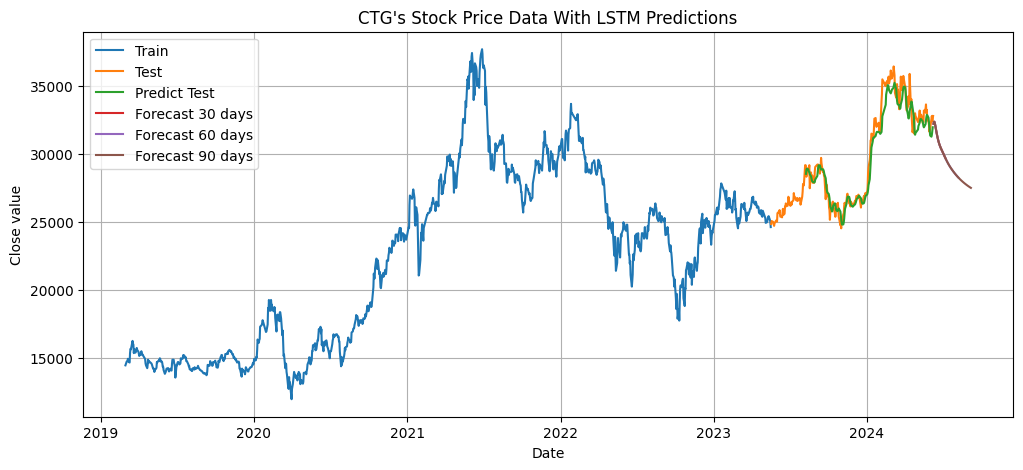
\includegraphics[width=\linewidth]{bibliography/CTG-LSTM-8-2.png}
    \caption{LSTM model's result with 8:2 splitting proportion}
    \label{fig8}
  \end{minipage}
\end{figure}
\begin{figure}[H]
  \centering
  \begin{minipage}{0.8\linewidth}
    \centering
    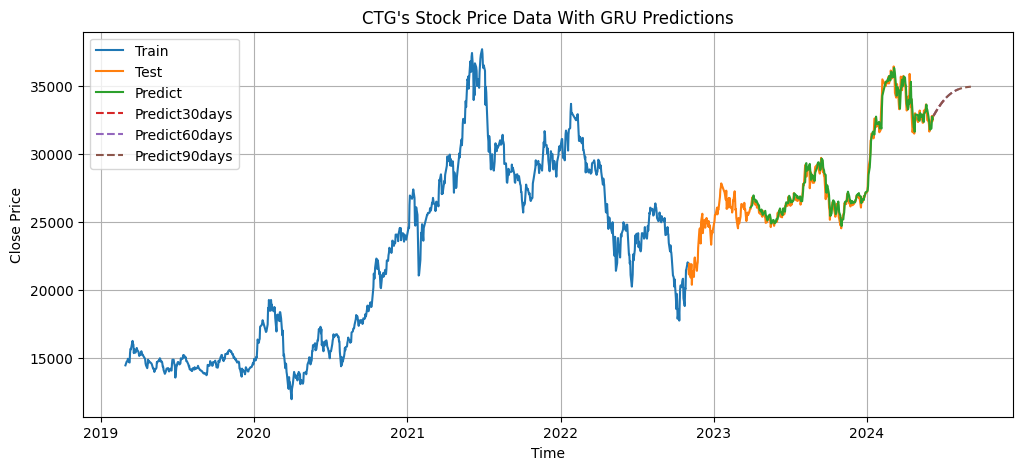
\includegraphics[width=\linewidth]{bibliography/CTG-GRU-7-3.png}
    \caption{GRU model's result with 7:3 splitting proportion}
    \label{fig8}
  \end{minipage}
\end{figure}
\begin{figure}[H]
  \centering
  \begin{minipage}{0.8\linewidth}
    \centering
    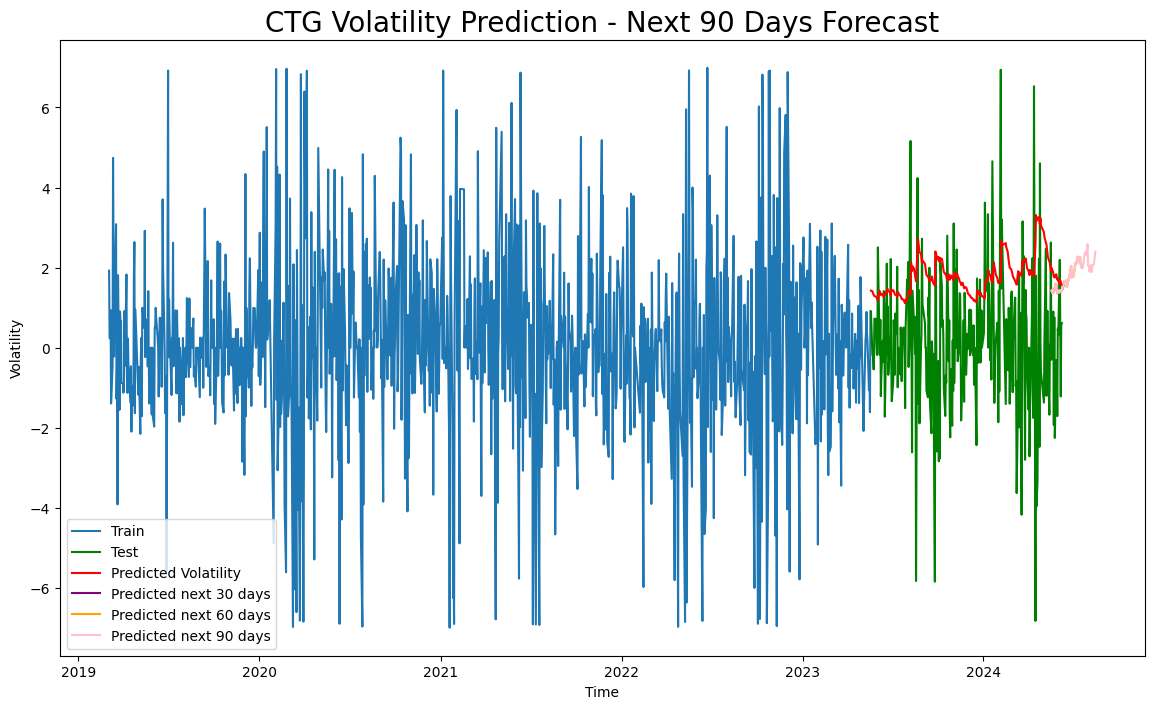
\includegraphics[width=\linewidth]{bibliography/CTG-GARCH-8-2.png}
    \caption{GARCH model's result with 8:2 splitting proportion}
    \label{fig8}
  \end{minipage}
\end{figure}
\begin{figure}[H]
  \centering
  \begin{minipage}{0.8\linewidth}
    \centering
    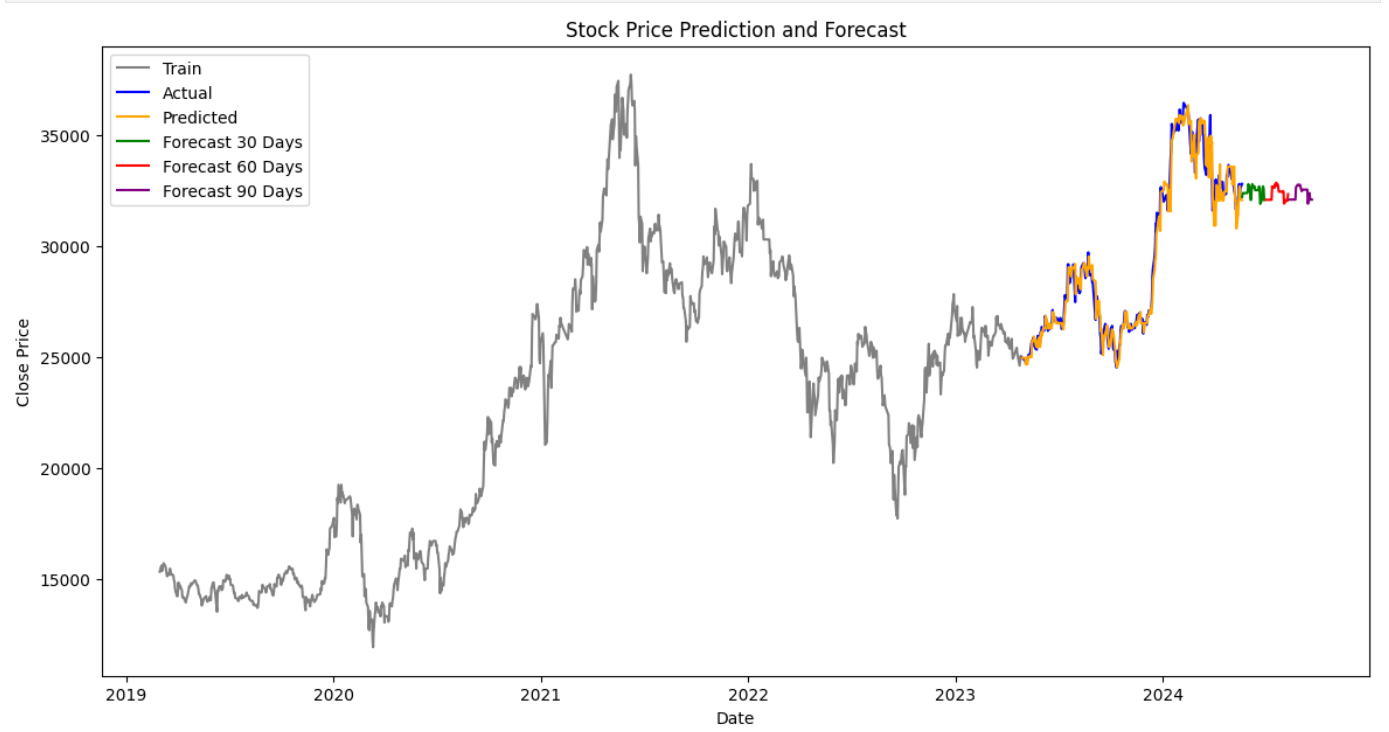
\includegraphics[width=\linewidth]{bibliography/CTG-GBR-8-2.png}
    \caption{GBR model's result with 8:2 splitting proportion}
    \label{fig25}
  \end{minipage}
\end{figure}
\begin{figure}[H]
  \centering
  \begin{minipage}{0.8\linewidth}
    \centering
    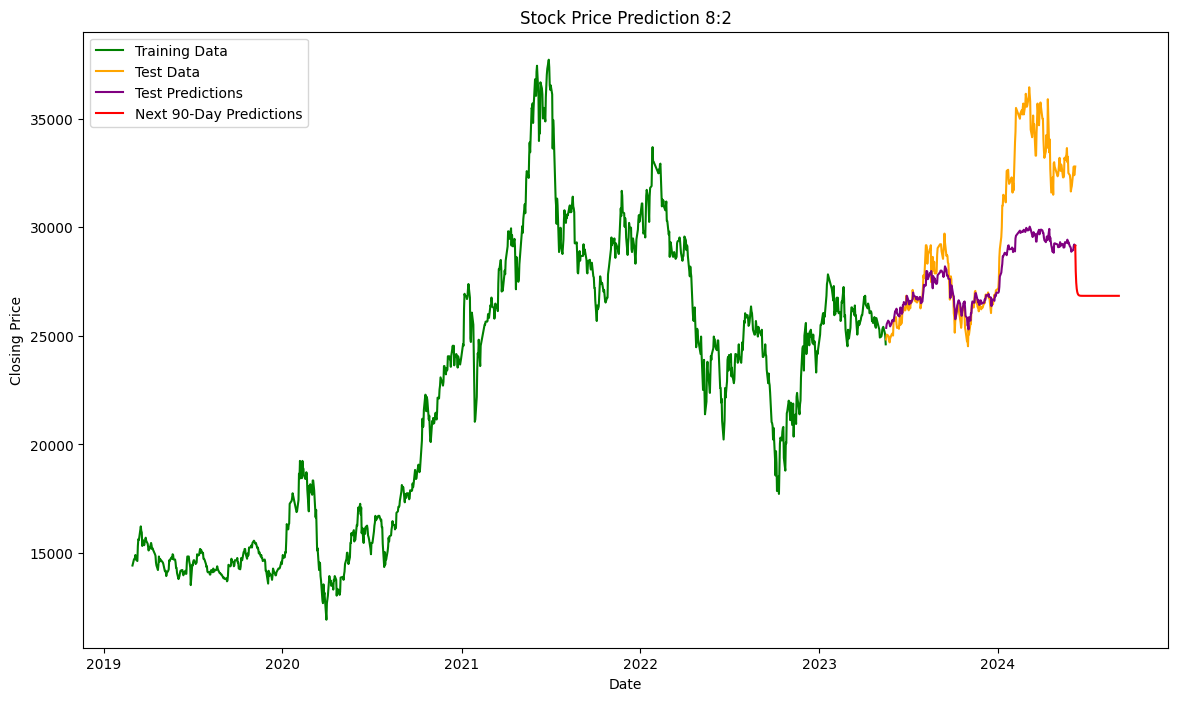
\includegraphics[width=\linewidth]{bibliography/CTG-MICN-8-2.png}
    \caption{MICN model's result with 8:2 splitting proportion}
    \label{fig26}
  \end{minipage}
\end{figure}

\section{Conclusion}
\subsection{Summary}
The results of this study highlight that out of the eight models tested (Linear Regression, ARIMA, RNN, LSTM, GRU, GARCH, GBR, and MICN), the GRU model emerged as the most suitable for predicting future values of VCB, ACB, and CTG bank stocks within the respective time series. This underscores the significant impact of algorithm selection on forecasting accuracy. Further development of deep learning algorithms in this area requires fine-tuning input parameters and expanding sample sizes. However, these efforts are challenged by the complex interplay of social variables that can drastically influence forecasting outcomes. Therefore, the findings presented here are for reference purposes and should be carefully considered in relation to specific research inquiries proposed by the investigator.
\section*{Acknowledgment}
\addcontentsline{toc}{section}{Acknowledgment}
First and foremost, we extend our heartfelt gratitude to \textbf{Assoc. Prof. Dr. Nguyen Dinh Thuan} for his invaluable guidance and enthusiastic support throughout this project. His lectures have provided our team with the knowledge and inspiration needed to successfully accomplish our goals. We would also like to express our sincere thanks to \textbf{Ms. Trinh Thi Thanh Truc} for her unwavering support during the course of this endeavor. We appreciate \textbf{Assoc. Prof. Dr. Nguyen Dinh Thuan} for granting us permission to undertake this project. Lastly, we deeply appreciate \textbf{Assoc. Prof. Dr. Nguyen Dinh Thuan}, \textbf{Ms. Trinh Thi Thanh Truc} and \textbf{Mr. Nguyen Minh Nhut} for their tireless efforts in guiding and encouraging our team every step of the way.


%% UNCOMMENT these lines below (and remove the 2 commands above) if you want to embed the bibliografy.
\begin{thebibliography}{00}
\bibitem{b1} Masoud, N. M. H. (2017). The impact of stock market performance upon economic growth. International Journal of Economics and Financial Issues, 3(4), 788-798.
\bibitem{b2} Murkute, A., and Sarode, T. (2015). Forecasting market price of stock using artificial neural network. International Journal of Computer Applications, 124(12), 11-15.
\bibitem{b3} Seber, G. A. F., and Lee, A. J. (2012). Linear regression analysis. John Wiley and Sons.
\bibitem{b4} Zhang, G. P. (2003). Time series forecasting using a hybrid ARIMA and neural network model. Neurocomputing, 50, 159-175.
\bibitem{b5} Li, L., Wu, Y., Ou, Y., Li, Q., Zhou, Y., and Chen, D. (2017). Research on machine learning algorithms and feature extraction for time series. In IEEE 28th Annual International Symposium on Personal, Indoor, and Mobile Radio Communications (PIMRC) (pp. 1-5). IEEE.
\bibitem{b6} Oyeyemi, E. O., McKinnell, L.-A., and Poole, A. W. V. (2007). Neural network-based prediction techniques for global modeling of M(3000)F2 ionospheric parameter. Advances in Space Research, 39(5), 643-650.
\bibitem{b7}Shen, G., Tan, Q., Zhang, H., Zeng, P., and Xu, J. (2018). Deep learning with gated recurrent unit networks for financial sequence predictions. Procedia Computer Science, 131, 895-903. https://doi.org/10.1016/j.procs.2018.04.298
\bibitem{b8}  Hochreiter, S., and Schmidhuber, J. (1997). Long short-term memory. Neural Computation, 9(8), 1735-1780. https://doi.org/10.1162/neco.1997.9.8.1735
\bibitem{b9} Hewamalage, H., Bergmeir, C., and Bandara, K. (2021). Recurrent neural networks for time series forecasting: Current status and future directions. International Journal of Forecasting, 37(1), 388-427. https://doi.org/10.1016/j.ijforecast.2020.06.008
\bibitem{b10} Chen, K., Zhou, Y., and Dai, F. (2015). A LSTM-based method for stock returns prediction: A case study of China stock market. In Proceedings of the 2015 IEEE International Conference on Big Data (Big Data), October 2015, Santa Clara, CA, USA (pp. 2823-2824). IEEE. https://doi.org/10.1109/BigData.2015.7364089
\bibitem{b11} Kim, J.-M., Kim, D. H., and Jung, H. (2021). Estimating yield spreads volatility using GARCH-type models. The North American Journal of Economics and Finance, 57, Article 100880. https://doi.org/10.1016/j.najef.2021.100880
\bibitem{b12} Agapitos, A., Brabazon, A., and O’Neill, M. (2017). Regularised gradient boosting for financial time-series modelling. Computational Management Science, 14, 367-391. https://doi.org/10.1007/s10287-017-0280-y
\bibitem{b13} Wang, H., Peng, J., Huang, F., Wang, J., Chen, J., and Xiao, Y. (2022, September). Micn: Multi-scale local and global context modeling for long-term series forecasting. In The Eleventh International Conference on Learning Representations.
\bibitem{b14} Vaswani, A., Shazeer, N., Parmar, N., Uszkoreit, J., Jones, L., Gomez, A. N., Kaiser, Ł., and Polosukhin, I. (2017). Attention is all you need. NeurIPS.
\bibitem{b15} Kumari, K., and Yadav, S. (2018). Linear Regression Analysis Study. Journal of the Practice of Cardiovascular Sciences, 4(1), 33. https://doi.org/10.4103/jpcs.jpcs-8-18
\bibitem{b16} Hyndman, R. J., and Athanasopoulos, G. (2021). Forecasting: Principles and practice. Melbourne: OTexts. Available at: https://otexts.com/fpp2/AR.html

\end{thebibliography}
%%%%%%%%%%%%%%%


\EOD

\end{document}
